\chapter{Métodos Estadísticos}

\section{Introducción}
El objetivo de todo estudio estadístico, es colectar datos y después usarlos para tomar una decisión. Cualquier decisión que se tome usando los resultados de un estudio estadístico es favorable cunado se usa un adecuado proceso de obtención de datos.
Si el proceso es defectuoso, entonces la decisión resultante es cuestionable.

\subsection{Pasos a tomar en cuenta en un estudio estadístico}

\begin{enumerate}
    \item Identificar la variable o variables de interés central y la población de estudio
    \item Desarrollar un plan detallado para colectar datos. Asegurar que los datos son representativos de la población
    \item Colectar los datos mediante un método de muestreo o diseño experimental.
    \item Describir el comportamiento de los datos obtenidos con técnicas de la estadística descriptiva (usar métodos gráficos y tabulares para condensar la información)
    \item Efectuar decisiones usando estadística inferencial. Identificar cualquier error posible.
\end{enumerate}

Existen varias formas que permiten colectar datos y muy a menudo el interés del estudio dicta la mejor vía para colectarlos.

\subsection{Los cuatro principales métodos de colección de datos}

\subsubsection{Desarrollar un experimento}

Cuando se desarrolla un experimento, un tratamiento es aplicado a parte de una población y las respuestas son observadas. Una segunda parte de la población es frecuentemente usada como control, este grupo no recibe tratamiento o se aplica un placebo.

Después de observar las respuestas en ambos grupos, los resultados son comparados (mediante una prueba de hipótesis estadística de interés).

\subsubsection{Usar simulación}

La simulación es el uso de modelos matemáticos o físicos para reproducir las condiciones de una situación o proceso.

Para la recolección de datos frecuentemente se involucra el uso de computadoras. La simulación permite estudiar situaciones que son peligrosas para llevarlos en un experimento y a menudo
traen un ahorro de tiempo y dinero para generar resultados.

\subsubsection{Toma de censos}

Un censo es un conteo o medición de la población entera de interés. Mediante el censo se obtiene información completa y detallada, pero frecuentemente es costoso y difícil de desarrollar.

\subsubsection{Usar muestreo}

El muestreo es un conteo o medición de una parte (usualmente pequeña) de una población. Las estadísticas calculadas a partir de una muestra son usadas para predecir varios parámetros poblaciones.

\begin{definition}[Muestra]
    Es una proporción de una población.
\end{definition}

\begin{definition}[Población]
    Una población consiste de todos los elementos (individuos u objetos) cuyas características deben ser estudiadas para un interés particular
\end{definition}

\begin{definition}[Censo]
    Es aquel estudio que incluye a cada miembro de la población
\end{definition}

\begin{definition}[Muestra representativa]
    Es aquella muestra que representa las características
\end{definition}

\begin{definition}[Elemento o miembro]
    Un elemento o miembro de una muestra o población es sujeto específico u objeto
\end{definition}

\begin{definition}[Variable]
    Es una característica bajo estudio que asume diferentes valores para diferentes elementos en contraste a una variable, el valor de una constante es fijo
\end{definition}

\begin{definition}[Variable cuantitativa]
    Es aquella variable que puede ser medida numéricamente
\end{definition}

\begin{definition}[Variable cualitativa]
    Es aquella variable que no puede ser medida numéricamente pero puede ser dividida en diferentes categorías.
\end{definition}

\begin{definition}[Observación o medición]
    El valor de una variable para un elemento
\end{definition}

\begin{definition}[Conjunto de dato]
    Observaciones sobre una o más variables
\end{definition}

Sobre las \textbf{Propiedades de los métodos}, proporcionan la máxima información contenida en los datos en forma árida y fácil de visualizar, poseen sencillez operativa y permiten presentar los datos de manera estética.

Dentro de los métodos \textbf{tabulares} y \textbf{gráficos}, permiten organizar y presentar datos de tal forma que los aspectos sobresalientes de los mismos son rápida y fácilmente aprensibles. En ocasiones estos métodos ayudan a establecer hipótesis sobre la naturaleza del fenómeno que se estudia.

En general, este tipo de tablas permite exhibir en forma concisa el número de veces que se presenta una determinada cantidad.

Sobre las \textbf{tablas de frecuencia} o \textbf{tablas de distribución de frecuencias}, se divide la amplitud de los valores numéricos de los datos en un cierto número de intervalos o clases, y se cuenta cuántas observaciones pertenecen a cada una de ellas.

\begin{definition}[Frecuencia]
    El número de observaciones que se pertenecen a una clase o intervalo
\end{definition}

El procedimiento de construcción de una tabla de frecuencias: se debe obtener el valor máximo y mínimo del conjunto de datos, se establece el ancho de clase. El ancho se obtiene al obtener la diferencia entre el valor máximo y mínimo, dividida por el número de clases y redondeando el número entero más cercano.

\begin{equation}
    \text{Ancho de clase}=\frac{\text{Valor máximo}-\text{Valor mínimo}}{\text{Número de clases}}
\end{equation}

Se establecen los valores límites de cada clase, el límite inferior de la clase define el valor más pequeño que puede contener la clase mientras que el límite superior define el valor más grande.

Use el menor valor presente en el conjunto de datos para definir el límite inferior de la primera clase y para


\begin{enumerate}
    \item Encontrar el valor medio de cada clase: el
          punto medio de una clase se obtiene al
          sumar el límite inferior de la clase al
          superior y dividido por dos. El punto
          medio es algunas veces llamado la marca
          de clase, se obtiene al aplicar la siguiente
          expresión.

          \begin{equation}
              \text{Punto medio}=\frac{\text{Límite Inferior+Límite Superior}}{2}
          \end{equation}

    \item Use marcas para indicar la pertenencia de un
          dato a una clase. Para evitar ambigüedades se
          dice que un dato pertenece a una determinada
          clase si su valor es estrictamente mayor que
          el límite inferior y menor o igual que el límite
          superior.

    \item Contar el número de marcas para encontrar la
          frecuencia total de cada clase denotada por fi
          Para encontrar la frecuencia relativa pi de
          cada clase se divide la frecuencia relativa de
          la i-ésima clase fi entre el total del número de
          datos.

          \begin{equation}
              p_1=\text{Frecuencia relativa}=\frac{\text{Frecuencia de clase}}{\text{Tamaño de muestra}}=\frac{f_i}{n}
          \end{equation}

\end{enumerate}

\begin{definition}[Frecuencia absoluta acumulada de una clase]
    Es la suma de las frecuencias absolutas de la
    clase y previas a la clase. La frecuencia
    acumulativa de la última clase es igual al
    tamaño de la muestra.
\end{definition}

\begin{definition}[Frecuencia relativa acumulada de una clase.]
    Se obtiene de manera similar a la frecuencia
    absoluta acumulada solo que en este caso se
    usan las frecuencias relativas. En este caso la
    frecuencia acumulativa de la última clase tiene
    el valor de uno.
\end{definition}

Finalmente, se elabora una interpretación de la información obtenida.

\subsubsection{Distribución de frecuencias}

\begin{enumerate}
    \item Decidir el número de clases
    \item Calcular el ancho de clase
    \item Determinar los límites de clase
    \item Marcar en la clase respectiva para cada valor
\end{enumerate}

%Histograma de frecuencias

\begin{definition}[Ojiva]
    permite obtener aquel número para el cual los valores del conjunto de datos son menores o iguales al valor, $x$ en un cierto porcentaje dado por la frecuencia relativa acumulada.
\end{definition}

\begin{definition}[Gráfica de pastel]
    Usada para describir partes de un todo ángulos centrales para cada segmento
\end{definition}
\begin{equation}
    \frac{\text{Número en categoría}}{\text{Número total}}\times360^{\circ}
\end{equation}

\subsection{Cálculo y selección de medidas descriptivas}

\subsubsection{Medidas de tendencia central}

\begin{definition}[Media]
    La suma de todos los datos divididos por el número de datos, para una población de muestra:
    \begin{equation}
        \mu=\frac{\sum_{j=1}^N X_i}{N}
    \end{equation}
\end{definition}

\begin{definition}[Mediana]
    El punto en el cual se tiene igual número de valores por arriba y por abajo.
\end{definition}

\begin{definition}[Moda]
    Es el número que tiene la mayor frecuencia
\end{definition}

\subsection{Medidas de dispersión}

La medida ponderada es aquella media de un conjunto de datos donde cada dato tiene diferentes pesos:

\begin{equation}
    \bar{x}=\frac{\sum_{i=1}^n x_i\cdot w_i}{\sum_{i=1}^n}w_i
\end{equation}

Donde $w_i$ es el peso de cada dato
\subsubsection{Medidas de variación }

El rango solo utiliza 2 números del conjunto de datos.

\begin{definition}[Desviación]
    La desviación para cada valor $x$ es la diferencia entre el
    valor de $x$ y la media del conjunto de datos.
\end{definition}

En una población, la desviación para cada valor de $x$ es $x-\mu$

En una muestra, la desviación para cada valor de x es $x-\hat{x}$

La suma de las desviaciones es 0

\begin{equation}
    \sum (x-\mu)=0
\end{equation}

\subsubsection{Varianza poblacional}

Varianza Poblacional: La suma de los cuadrados
de las desviaciones, dividida por N.

\begin{equation}
    \sigma^2=\frac{\sum (x-\mu)^2}{N}
\end{equation}

\subsubsection{Desviación estándar poblacional}

La desviación estándar poblacional es la raíz cuadrada
de la varianza poblacional.


\begin{equation}
    \sigma=\sqrt{\sigma^2}
\end{equation}

\subsubsection{Desviación estándar muestral}

Para calcular la varianza muestral, la suma de los
cuadrados de las desviaciones se divide por $n-1$.

La desviación estándar muestral, $s$ se calcula al obtener la raíz
cuadrada de la varianza muestral.

\begin{equation}
    s^2=\frac{\sigma^2}{n-1}
\end{equation}

\subsubsection{Coeficiente de variación}

\begin{equation}
    CV=frac{s_x}{\bar{x}}\times 100
\end{equation}

Puesto que tanto la desviación estándar como la
media se miden en las unidades originales, el \textbf{CV} es
una medida independiente de las unidades de
medición.

Debido a la anterior propiedad, el CV es la cantidad
más adecuada para comparar la variabilidad de dos
conjuntos de datos.

En áreas de investigación donde se tienen datos de
experimentos previos, el CV es muy usado para
evaluar la precisión de un experimento, comparando
el CV del experimento en cuestión con los valores
del mismo en experiencias anteriores.

\begin{example}

    Para los datos de los precios de los dos lotes de producto al
    cierre de diez días de ventas, se tiene que:
    $S_A=4.57651$ y $S_B=18.31362$, donde la media es la misma
    =61.5, por lo tanto:
    \begin{align*}
         & \text{CV(Lote A)}=\frac{4.57651}{61.5}\times 100=7.44\%   \\
         & \text{CV(Lote B)}=\frac{18.31362}{61.5}\times 100=29.77\%
    \end{align*}
\end{example}


Puede verse claramente a partir de lo anterior, que los
datos que corresponden al lote $B$ tienen una mayor
variabilidad que los que pertenecen al lote A.

Los datos con distribución simétrica en forma de campana tienen
las siguientes características.

\begin{figure}[h!]
    \centerline{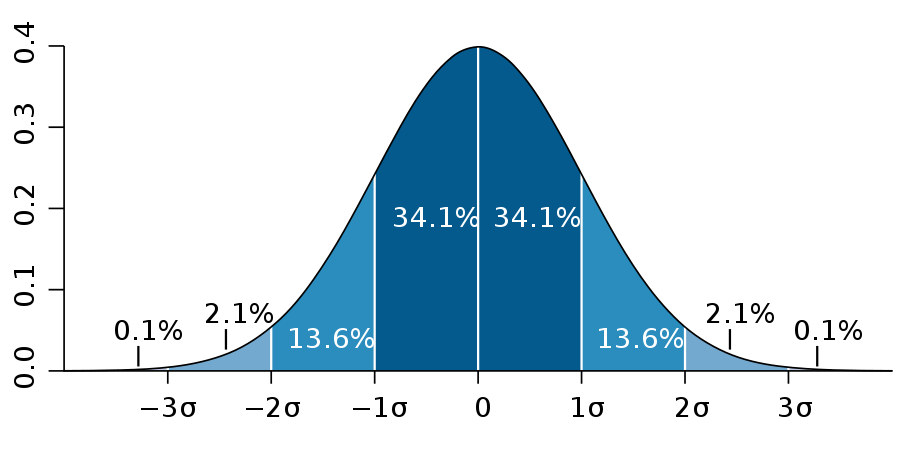
\includegraphics[width=0.5\textwidth]{me1.png}}
    \caption{Regla 68- 95- 99.7\%}
    \label{me1}
\end{figure}

\begin{enumerate}
    \item Cerca del 68\% de los datos quedan comprendidos dentro de una
          desviación estándar con respecto a la media
    \item Cerca del 99.7\% de los datos se encuentra dentro de tres desviaciones
          estándar
    \item Cerca del 95\% de los datos quedan comprendidos dentro de dos
          desviaciones estándar.
\end{enumerate}

\begin{theorem}[Teorema de Chebyshev]
    Para cualquier distribución independientemente de su forma, la
    proporción de datos que caen dentro de $k$ desviaciones
    estándar $(k >1)$ con respecto a la media es al menos $1-\frac{1}{k^2}$.

    \begin{enumerate}
        \item Para $k = 2$, al menos $1-\frac{1}{4} = \frac{3}{4}$ o $75\%$ de los datos caen
              dentro de 2 desviaciones estándar de la media.
        \item Para $k = 3$, al menos$ 1-\frac{1}{9} = \frac{8}{9}= 88.9\%$ de los datos quedan
              comprendidos dentro de 3 desviaciones estándar con respecto
              a la media.
    \end{enumerate}
\end{theorem}

\emph{El teorema de Tchebychev permite inferir la proporción de valores que deben quedar dentro de una cantidad específica de desviaciones estándar respecto a la media}

Para aproximar la media de un conjunto de datos presentados
en una distribución de frecuencia, se considera como si los
valores de cada clase ocurrieran en el punto medio de su clase.
$x=$ Punto medio de la clase.

\begin{equation}
    \bar{x}=\frac{\sum (x\cdot f)}{n}
\end{equation}

\subsubsection{Mediana}

Para calcular la mediana en una tabla de
frecuencias procédase como sigue:

\begin{enumerate}
    \item Localízate la clase de la mediana. Ésta es
          una clase tal que la frecuencia relativa
          acumulada hasta la clase que le precede, y la
          frecuencia relativa acumulada hasta ella, son
          respectivamente menor que, y mayor o igual
          a 0.5.

    \item Calcúlese la mediana mediante la ecuación:
          \begin{equation}
              Me=a+\frac{(b-a)(0.5-c)}{(d-c)}
          \end{equation}

          Donde $a=$Límite inferior de la clase de la mediana,
          $b=$Límite superior de la clase de la mediana,
          $c=$Frecuencia relativa acumulada hasta la clase que precede a la de la mediana,
          $d=$Frecuencia relativa acumulada de la clase de la mediana.
\end{enumerate}

\subsubsection{Moda}

Si es un valor único se dice que la distribución de frecuencias es unimodal.

Si se tienen dos o más valores con la misma frecuencia máxima se dice que la distribución es bimodal, trimodal,
etc.

\subsubsection{las medidas de tendencia central}

\begin{enumerate}
    \item Si la distribución no es muy asimétrica, la moda, media y
          mediana tienen aproximadamente el mismo valor, por lo
          que puede reportarse cualquiera de la tres,
    \item Para distribuciones asimétricas, la mediana puede ser mejor
          medida de tendencia central,
    \item Si va a procederse a hacer estadística inductiva, la media es
          indispensable por sus excelentes propiedades teórica que se
          verán posteriormente,
    \item Si se trata sólo de describir un conjunto, es conveniente
          reportar las tres medidas, ya que cada una puede indicar más
          información al investigador.
\end{enumerate}

Para calcular la varianza en una tabla de
frecuencias se opera bajo las mismas
suposiciones que, en el caso de la media, por
lo tanto se tiene:

\begin{equation}
    s^2=\left(\frac{1}{n-1}\right)\sum_{i=1}^{k}\left(x_i-\bar{x}\right)^2\left(f_i\right)
\end{equation}

ó también se puede emplear:

\begin{equation}
    s^2=\left(\frac{1}{n-1}\right)\left[ \sum_{i=1}^{k}x_i^2f_i-\frac{\left(\sum_{i=1}^{k}x_if_i\right)}{2} \right]
\end{equation}

Para aproximar la desviación estándar de los datos en una distribución de frecuencias, se usa $x_i$= \textbf{punto medio} de la clase.

\begin{equation}
    s=\sqrt{\frac{\sum \left(x-\bar{x}\right)^2f}{n-1}}
\end{equation}

\begin{example}
    \begin{table}[h!]
        \centering
        \begin{tabular}{@{}lllll@{}}
            \toprule
            Clase   & $f$ & $x_i$ & $\left(x-\bar{x}\right)^2$ & $\left(x-\bar{x}\right)^2f$ \\ \midrule
            67- 78  & 3   & 72.5  & 739.84                     & 2219.52                     \\
            79- 90  & 5   & 84.5  & 231.04                     & 1155.20                     \\
            91- 102 & 8   & 96.5  & 10.24                      & 81.92                       \\
            103-114 & 9   & 108.5 & 77.44                      & 696.96                      \\
            115-126 & 5   & 120.5 & 432.64                     & 2163.2                      \\
                    & 30  &       &                            & 6316.8                      \\ \bottomrule
        \end{tabular}
        \caption{ Ejemplo de cálculo de varianzas}
        \label{tabme1}
    \end{table}

    Aplicando la fórmula, se obtiene la varianza:

    \begin{equation*}
        s=\sqrt{\frac{6316.8}{29}}=\sqrt{217.8207}=14.76
    \end{equation*}
\end{example}

\subsubsection{Medidas de dispersión}

Las tres medidas de dispersión que se usan en la práctica
son el rango, la desviación estándar y el coeficiente de
variación.

\begin{enumerate}
    \item El rango o amplitud se usa por ser muy fácil de calcular. Por
          estar basada sólo en dos valores, es la medida de dispersión
          más sensible a observaciones extremas.
    \item La desviación estándar tiene las ventajas y desventajas de la
          media muestral. Es indispensable en estadística inductiva.
    \item Por ser independiente de las unidades de medición, el
          coeficiente de variación es la medida apropiada para
          comparar la variabilidad de dos conjuntos de datos.
\end{enumerate}

\subsubsection{Cuartiles}

Tres cuartiles $Q_1$, $Q_2$ and $Q_3$ dividen los datos en cuatro partes iguales.

\begin{itemize}
    \item $Q_2$ es lo mismo que la mediana.
    \item $Q_1$ es la mediana de los datos abajo de $Q_2$
    \item $Q_3$ es la mediana de los datos arriba de $Q_2$
\end{itemize}

A continuación se muestran los datos que
corresponden al número de aspersores vendidos en
27 días del año seleccionados de manera aleatoria
para una empresa de riego. Encontrar $Q_1$, $Q_2$ y $Q_3$\dots

28 43 48 51 43 30 55 44 48 33 45 37 37 42
27 47 42 23 46 39 20 45 38 19 17 35 45

Los datos ordenados $(n = 27)$ son:

17 19 20 23 27 28 30 33 35 37 37 38 39 42 42
43 43 44 45 45 45 46 47 48 48 51 55

Rango medio $\frac{27+1}{2} = 14$. La mediana =$Q_2$= 42.

Existen 13 valores abajo de la mediana.
$Q_1$ rango = 7. $Q_1$ es 30.
$Q_3$ es el rango 7 contando desde el último valor.
$Q_3$ es 45.

\begin{remark}
    El rango Intercuartil es $Q_3-Q_1=45-30=15$
\end{remark}

\subsubsection{ Gráfica de cajas y ejes}


Se construye a partir del uso de 5 valores claves para describir un
conjunto de datos. $Q_1$, $Q_2$ y $Q_3$, el valor mínimo y máximo.

\begin{align*}
     & Q_1                   &  & 65  \\
     & Q_2=\text{la mediana} &  & 80  \\
     & Q_3                   &  & 115 \\
     & \text{Valor mínimo}   &  & 55  \\
     & \text{Valor Máximo}   &  & 120
\end{align*}

\begin{figure}[h!]
    \centering
    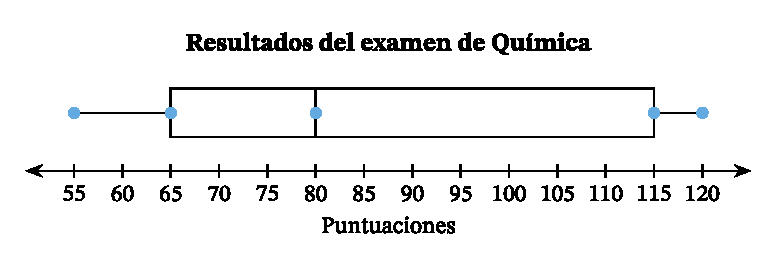
\includegraphics[scale=0.5]{es2.pdf}
    \caption{Gráfica de cajas y ejes}
\end{figure}

\subsubsection{Percentiles}

Los percentiles dividen los datos en 100 partes iguales. Hay 99 percentiles: $P_1, P_2, P_3\dots P_99$.

\begin{align*}
    P_{25}=Q_1 &  & P_{50}=Q_2=\text{la mediana} &  & P_{75}=Q_3
\end{align*}

El $63^{\circ}$ percentil indica aquel valor del conjunto de
datos para el cual se cumple que el 63\% de las
observaciones o datos son menores o iguales y
37\% de los datos son superiores a ese valor.

\begin{figure}[h!]
    \centering
    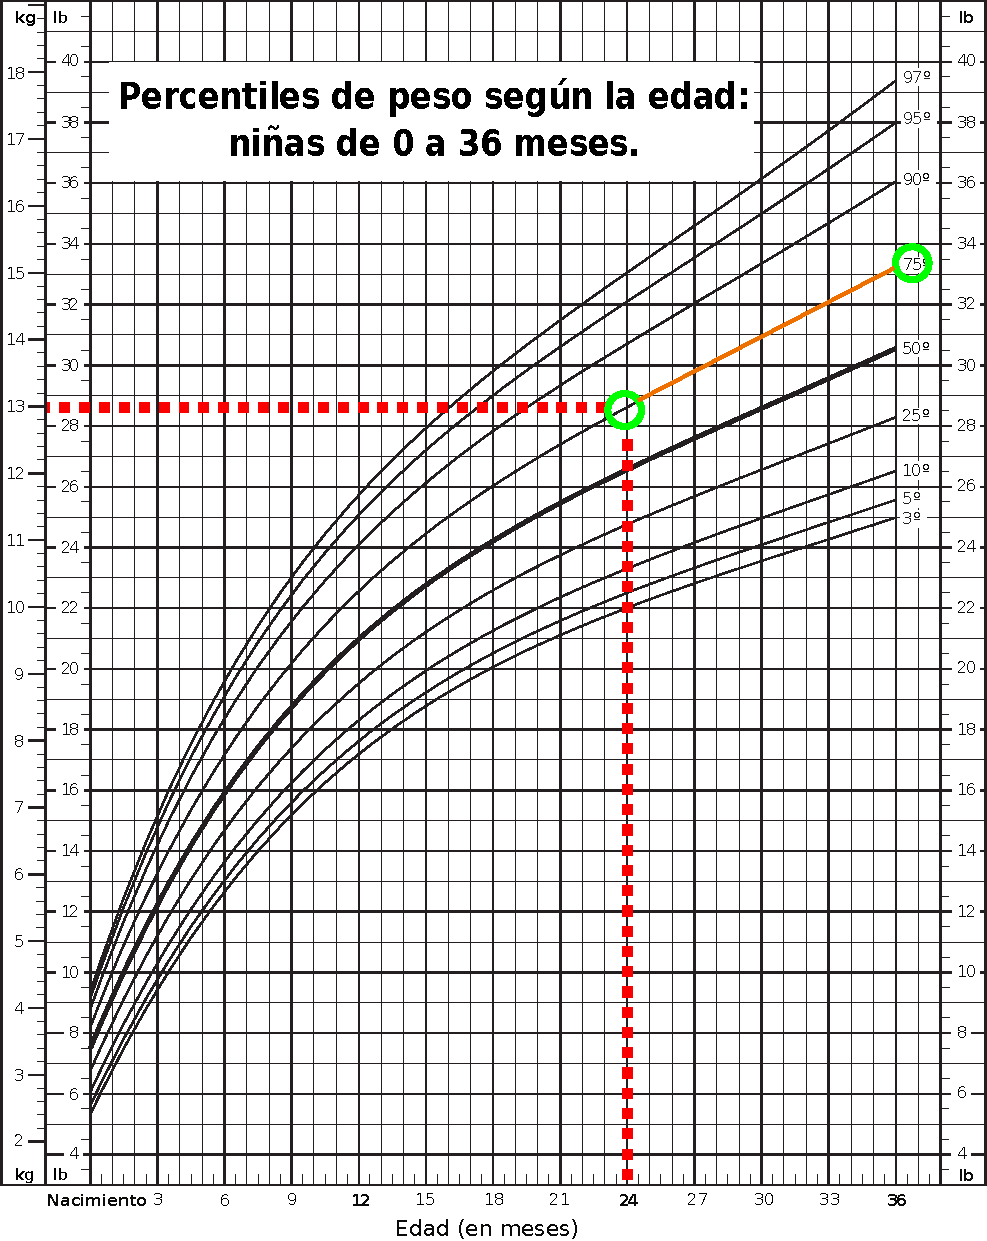
\includegraphics[scale=0.5]{es3.pdf}
    \caption{Percentiles}
\end{figure}

La distribución acumulativa puede ser usada para encontrar
los percentiles.


Para el valor de 24 se tiene que 13 de los 18 valores se encuentran por abajo, es decir $13/18 = 72.22\%$. Se puede aproximar a $24=P_{72}$.

\subsection{Descripción simultánea de dos conjuntos de datos.}

Cuando se estudian dos características, una pregunta que
surge con frecuencia es si existe alguna relación entre ellas,
A continuación se presentan dos medidas que son útiles para
describir el grado de asociación entre dos conjuntos de datos.

\begin{definition}[Covarianza $S_{xy}$]
    Sean $(x_1,y_1),(x_2,y_2),\dots,(x_n,y_n)$ $n$ pares de observaciones de dos características $X$ y $Y$. sean $\bar{x}\land \bar{y}$ Sus respectivas medias muestrales.
    La covarianza entre las dos características se define como:
    \begin{equation}
        s_{xy}=\frac{1}{n-1} \sum_{i=1}^{k}\left(x_i-\bar{x}\right)\left(y_i-\bar{y}\right)
    \end{equation}
\end{definition}

La ecuación para calcular la covarianza de una población de tamaño $N$ es la siguiente:

\begin{equation}
    \sigma_{xy}=\frac{\sum_{i=1}^{n} \left(x_i-\mu_{x}\right)\left(y_i-\mu_{y}\right)}{N}
\end{equation}

Otra expresión equivalente para $S_{XY}$

\begin{equation}
    \sigma_{xy}=\frac{1}{n-1}\left[ \sum_{i=1}^{n}x_iy_i-\frac{\left(\sum_{i=1}^{n}x_i\right)\left(\sum_{i=1}^{n}y_i\right)}{n} \right]
\end{equation}

\subsubsection{Propiedades de la covarianza}

Cuando los valores de la variable X crecen con
los de la variable Y, la covarianza es positiva.

Cuando los valores de la variable X decrecen al
aumentar los de la variable Y, la covarianza es
negativa.

Al comparar las ecuaciones que sirven para el
cálculo de la covarianza SXY y de la varianza ,
se puede observar que la expresión para calcular la
varianza se obtiene al obtener la covarianza de la
misma variable X, es decir se puede ver a la
varianza como un caso particular de la covarianza.

La covarianza como medida de asociación entre dos
variables depende de las unidades en que se miden
las variables de interés.

No existen valores de referencia que indiquen el
grado de asociación entre las dos variables, solo que
entre más alejados de cero indica mayor asociación
lineal.

\begin{definition}[Definición de correlación $r_{XY}$]
    Sean $(x_1,y_1), (x_2,y_2),\dots,(x_n,y_n)$ $n$ pares de observaciones
    hechas de dos características $X$ y $Y$, sean $\bar{x}\land \bar{y}$ Sus respectivas medias muestrales.

    $S_{XY}$ La covarianza entre las dos características, El coeficiente de correlación $r_{XY}$, o simplemente la correlación
    entre las dos variables, tiene como expresión:

    \begin{equation}
        r_{XY}=\frac{S_{XY}}{S_{X}\cdot S_{Y}}
    \end{equation}
\end{definition}

De manera más explícita se tiene:

\begin{equation}
    r_{XY}= \frac{\left[\sum_{i=1}^n x_i\cdot y_i-\frac{\left(\sum_{i=1}^n x_i\right)\left(\sum_{i=1}^n y_i\right)}{n}\right]}{\left\{\left[\sum_{i=1}^n x_i^2-\frac{\left(\sum_{i=1}^n x_i\right)^2}{n}\right]\cdot\left[\sum_{i=1}^n y_i^2-\frac{\left(\sum_{i=1}^n x_i\right)^2}{n}\right]\right\}}^{12}
\end{equation}

\subsubsection{Propiedades de la correlación}

Es independiente de las medidas utilizadas en las
variables.

Valores positivos del coeficiente indican que las
variables tienden a crecer (o decrecer)
simultáneamente, y valores negativos indican que
una aumenta cuando la otra disminuye.

Toma valores exclusivamente entre -1 y 1. Entre más cercano se encuentre el valor de la
correlación a -1 ó +1 más fuerte la asociación lineal
entre las dos variables y valores cercanos a cero
indican una pobre asociación lineal.


\section{Probabilidad}

\begin{definition}[Experimento]
    Es un proceso mediante el cual se obtiene una observación o medición.
    Durante gran parte de las prácticas que se desarrollan en algunas materias, el estudiante obtiene observaciones, con lo cual es posible verificar alguna ley física.
\end{definition}

\begin{definition}[Experimento aleatorio]
    Es aquel cuyos resultados no pueden predecirse antes de su realización, por lo tanto están sujetos al azar, por ejemplo:
    \begin{itemize}
        \item Lanzar una moneda
        \item El sexo de un bebé que está por nacer
        \item El valor del tirante en un canal de riego en un día del año
        \item El número de semillas sembradas y que podrán germinar y emerger
        \item El color de un jitomate creciendo dentro de un invernadero
    \end{itemize}
\end{definition}


\begin{definition}[Espacio muestral]
    Es el conjunto integrado por todos los resultados
    posibles de un experimento y se denota por la letra $M$
\end{definition}

En función de los elementos que conforman el
espacio muestral se distinguen dos tipos:


\begin{enumerate}
    \item \textbf{Espacio muestral discreto:} Es aquel que está
          formado o integrado por elementos que pueden
          numerarse por un número finito o infinito
          denumerable.
    \item Espacio \textbf{muestral continuo:} Es aquel que
          contiene todos los elementos en uno o varios
          segmentos de la línea recta real\footnote{Un espacio muestral no necesariamente está
              integrado por números, también puede contener
              mediciones cualitativas.}.
\end{enumerate}

\begin{definition}[Partición del espacio muestral]
    Si el espacio muestral se divide en cierto número de
    eventos, denotados por $A_1,A_2\dots A_K$ de tal manera que se
    cumple que:

    \begin{itemize}
        \item $A_i \cap A_j=\varnothing$, para cualquier par de eventos (es decir, que los
              eventos sean mutuamente excluyentes)
              $A_1 \cup A_2 \cup\dots \cup A_k =M$, es decir la unión de todos los eventos
              es igual al espacio muestral.
    \end{itemize}
    Se dice que se tiene una partición del espacio muestral.
\end{definition}

\begin{definition}[Probabilidad]
    La probabilidad de un evento $A$, es un número real en el intervalo [0,1], que denotaremos por $P(A)$
    y representa una medida de la \textit{frecuencia} con la que se observa la ocurrencia del evento $A$ cuando se efectúa el experimento aleatorio en cuestión.
\end{definition}

\begin{definition}[Probabilidad clásica]
    Sea $A$ un subconjunto de un espacio muestral $\Omega$ de cardinalidad finita. Se define la probabilidad clásica del evento $A$ como el cociente:
    \begin{equation}
        P(A)=\frac{\#A}{\#\Omega}
    \end{equation}
\end{definition}

Donde:
$\# A$, denota la cardinalidad del conjunto $A$
$\# \Omega$, denota la cardinalidad del espacio muestral

Claramente esta definición es sólo válida para espacios
muestrales finitos, pues forzosamente necesitamos
suponer que el número de elementos en $\Omega$ es finito.

Además, el espacio $\Omega$ debe ser equiprobable, pues para
calcular la probabilidad de un evento $A$, únicamente
necesitamos contar cuántos elementos tiene $A$ respecto del
total $\Omega$, sin importar exactamente qué elementos
particulares sean. Por lo tanto, esta definición de probabilidad presupone que
todos los elementos de $\Omega$ son igualmente probables o
tienen el mismo peso.

En algunos problemas del cálculo de probabilidades se
dificulta el cálculo de la cardinalidad de los eventos
definidos y del espacio muestral. Puede usarse algunas técnicas de conteo como son la
combinaciones y permutaciones.

\subsubsection{Análisis combinatorio}

\begin{definition}[Principio de multiplicación]
    El principio de multiplicación que se enuncia a
    continuación es la base de muchos de los cálculos en las
    técnicas de conteo. Si un procedimiento puede efectuarse de $n$ formas
    distintas y un segundo procedimiento puede realizarse de
    $m$ formas diferentes, entonces el total de formas en que
    puede efectuarse el primer procedimiento seguido del
    segundo es el producto $n\cdot m$
\end{definition}

\FrameTBStyle{c}
\begin{lstlisting}[style=cFrameTB, gobble=4]
        #include <stdio.h>
        #include <stdlib.h>
        // Programa para mostrar todas las posibles combinaciones 
        con lo numeros del dado y las letras del abecedario
        int main(){
            int i,I=0;
            char j;
                printf("Hello world!\n");
                for(i=1;i<=6;i++)
                for(j=97;j<123;j++) //las letras del abecedario inician en 97
                {
                printf("(%d,%c)\n",i,j); // Se imprimen tanto el numero como la letra del abecedario
                I++;
                }
                printf("Valor de I=%d\n",I);
                return 0;
        }
    \end{lstlisting}

El principio de multiplicación es válido no solamente para
dos procedimientos sino que también vale para cualquier
sucesión finita de procedimientos. Por ejemplo:

$A_1,A_2\dots A_K$ denotan $k$ procedimientos sucesivos
entonces el principio de multiplicación se puede enunciar
en símbolos de la forma siguiente:


\begin{equation*}
    \# (A_1\times \dots \times A_N)=\# A_1\dots \# A_K
\end{equation*}

\begin{definition}[Probabilidad frecuentista]
    Supongamos que realizamos n veces un cierto experimento
    aleatorio y sea $A$ un evento cualquiera.

    Denotemos por $n(A)$ el número de ocurrencias del evento A,
    en las $n$ realizaciones del experimento. Se define entonces la
    probabilidad frecuentista de $A$ como indica el siguiente límite
\end{definition}
\begin{equation}
    P(A)=\lim_{n\to \infty} \frac{n(A)}{n}
\end{equation}

En este caso, debemos hacer notar que no es humanamente
posible llevar a cabo una infinidad de veces el experimento
aleatorio, de modo que en la práctica no es posible encontrar
mediante este mecanismo la probabilidad de un evento
cualquiera.

Esta limitación hace que esta definición de probabilidad no
sea enteramente formal, pero tiene algunas ventajas.

\begin{definition}[Probabilidad subjetiva]
    En este caso la probabilidad de un evento depende del
    observador, es decir, según lo que el observador conoce
    del fenómeno en estudio.
\end{definition}

Puede parecer un tanto informal y poco serio esta forma
de definir la probabilidad de un evento, sin embargo en
muchas situaciones prácticas es necesario recurrir a un
experto para tener por lo menos una idea vaga de cómo
se comporta el fenómeno de nuestro interés y saber si la
probabilidad de un evento es alta o baja.


\begin{definition}[Probabilidad axiomática]
    Se proponen las reglas que el cálculo de
    probabilidades debe satisfacer. Los siguientes son tres
    postulados o axiomas establecidos en 1933 por el
    matemático ruso A. N. Kolmogorov
\end{definition}


\subsubsection{Axiomas de la probabilidad}

\begin{enumerate}
    \item $P(A)\geq 0$
    \item $P(\Omega)=1$
    \item $P(A\cup B)=P(A)+P(B) \text{Cuando } A\cup B=\varnothing$
\end{enumerate}

No es difícil verificar que las definiciones anteriores de
probabilidad satisfacen estos tres axiomas. De hecho, estos
postulados han sido tomados directamente del análisis
cuidadoso y reflexivo de las definiciones de probabilidad
mencionadas anteriormente. En particular observe que el
tercer axioma es válido no sólo para dos eventos ajenos
sino para cualquier colección finita de eventos ajenos dos a
dos.

A cualquier función P que satisfaga los tres axiomas de
Kolmogorov se le llama medida de probabilidad, o
simplemente probabilidad. Como consecuencia de estos
postulados es posible demostrar que la probabilidad cumple,
entre otras, con las siguientes propiedades

\begin{example}
    Sabiendo que los eventos $A$ y $A^C$ son una partición del
    espacio muestral, es decir cumplen con $A\cup A^C =M$ y $A \cap A^C =\varnothing$.

    Entonces por el axioma uno: $P(M)=1$, Por el axioma tres. $P(A\cup A^C )=P(A)+P(A^C)$,
    de donde $P(M)=1=P(A)+P(A^C) \implies P(A^C)=1-P(A)$
\end{example}


Algunas propiedades de la propiedad son:

\begin{align*}
    & P(A^C)=1-P(A)                                                                     \\ &P(\varnothing)=0\\ &A\subseteq B \implies P(A)\leq P(A)\\
    & A\subseteq B \implies P(B-A)=P(B)-P(A)                                            \\&0\leq P(A) \leq 1\\& P(A\cup B)=P(A)+P(B)-P(A\cap B)\\
    & P(A\cup B\cup C)=P(A)+P(B)+P(C)-\dots\\
    &\dots P(A\cap B)-P(A\cap C)-P(B\cap C)+P(A\cap B\cap C)
\end{align*}

%%%%%%%%%%%%%%%%%%%%%%%%%%%%%%%%%%%%%%%%%%%%%%%%%%%%%%%%%%%%%%%%%%%%%%%%%%%%%%%%%%%%%%%
%%%%%%%%%%%%%%%%%%%%%%%%%%%%%%%%%%%%%%%%%%%%%%%%%%%%%%%%%%%%%%%%%%%%%%%%%%%%%%%%%%%%%%%


\subsection{Probabilidad condicional e independencia}
Sean $A$ y $B$ dos eventos en donde $P (B) > 0$. La probabilidad
condicional del evento $A$ dado el evento $B$, denotada por $P(A\mid B)$, se
define como sigue:

\begin{equation}
    P(A\mid B)=\frac{P(A\cap B)}{P(B)}
\end{equation}


La expresión $P(A\mid B)$ se lee entonces ``probabilidad condicional del
evento $A$ dado que ocurrió el evento $B$'' o simplemente ``probabilidad
de $A$ dado $B$''. Para que la definición tenga sentido se necesita suponer
que $P(B) > 0$. No se define $P (A\mid B)$ cuando $P (B) = 0$.

El evento $B$ representa información adicional acerca del experimento
aleatorio. Mediante un ejemplo sencillo se ilustra a continuación el uso
y significado de la probabilidad condicional


\begin{example}
    Considere el experimento de lanzar un dado equilibrado.
    Donde $\Omega= \left\{ 1, 2, 3, 4, 5, 6 \right\}$ el cual es equiprobable.
\end{example}

\textit{ Sol. }

Sean los eventos $A=\left\{2\right\}$  y $B=\left\{2, 4, 6\right\} =$  ``Ocurre un número par''.
Note que el evento $A$ dado $B$ denotado por $A\mid B$, en palabras quiere
decir ocurre el número 2 dado que ocurrió un número par y en
términos de probabilidad condicionada se tiene simbólicamente

\begin{equation}
    P( A\mid  B)=\frac{P( A\cap B)}{P(B)}
\end{equation}

Note que$ A\cap B= \left\{2\right\}\cap \left\{2,4,6\right\}=\left\{2\right\}$, por lo tanto $P(\left\{2\right\})=\frac{1}{6}$ y como
$P(B)=P(\left\{2,4,6\right\})=\frac{3}{6}=\frac{1}{2}$, entonces.

\begin{equation*}
    P( A\mid  B)=\frac{\frac{1}{6}}{\frac{1}{2}}=\frac{2}{6}=\frac{1}{3}
\end{equation*}

Note, como se incrementa la probabilidad de que ocurra el número 2,
al saber que se tiene información de que ha ocurrido un número par.



\subsection{Independencia de dos eventos}

Cuando dos eventos son independientes, es decir, si la
probabilidad del evento $B$ es igual, ya sea que el evento A
haya o no ocurrido, entonces el evento $A$ no afecta al
evento $B$ y por tanto:

\begin{equation}
    P( A\mid  B)=\frac{P( A\cap B)}{P(B)}=P(A)
\end{equation}


\subsubsection{La regla de la multiplicación para eventos independientes}

Si dos eventos $A$ y $B$ son independientes, la probabilidad
de que ocurran $A$ y $B$ es:

\begin{equation}
    P(A \cap B) =P(A)\cdot P(B)
\end{equation}

Del mismo modo, si $A$, $B$ y $C$ son eventos mutuamente
independientes (todos los pares de eventos son
independientes), entonces la probabilidad de que $A$, $B$ y $C$
ocurran es:

\begin{equation}
    P(A \cap B \cap C)= P(A)\cdot P(B)\cdot P(C)
\end{equation}


\subsubsection{Verificación de independencia}

Se dice que dos eventos $A$ y $B$ son independientes si y sólo si $P(A \cap B)=P(A)\cdot P(B)$
o bien, $P(B \mid  A) =P(B)$ o, en forma equivalente, $P(A \mid  B) = P(A)$
De otro modo, se dice que los eventos son dependientes.


\begin{example}
    Sea el experimento que consiste en lanzar al aire dos monedas y
    observar el resultado que aparece en las dos monedas. Defina estos
    eventos:
    \begin{enumerate}
        \item Águila en la primera moneda
        \item Sello en la segunda moneda
    \end{enumerate}

    ¿Los eventos $A$ y $B$ son independientes?
\end{example}

\textit{ Sol. }

En este caso primero se estudia el espacio muestral que al analizar los resultados posibles en cada lanzamiento es:

\begin{equation*}
    M = \Omega  = \left\{(AA),(AS),(SA),SS\right\}
\end{equation*}

Si se asume que todos los eventos son igualmente probables, entonces se tiene
que, de la definición clásica de probabilidad:

\begin{equation*}
    P(AA)=P(AS)=P(SA)=P(SS)=\frac{1}{4}
\end{equation*}

Por otra parte asumiendo que $P(A)=P(S)=\frac{1}{2}$ en cada lanzamiento.
Note que en este caso, los eventos que cumple con los eventos ya definidos:

\begin{enumerate}
    \item $A:$ Águila en la primera moneda $\implies  \left\{AA\right\} y \left\{AS\right\}$
    \item $B:$ Sello en la segunda moneda  $\implies  \left\{AS\right\}$
\end{enumerate}

En este caso $A \cap B =( {AA}, {AS} )\cap( {AS} )={AS}$

Por lo tanto:

\begin{equation*}
    P( A\cap B)=\frac{\# ( A\cap B)}{\#\Omega}=\frac{\#( AS)}{\#( AA , AS ,SA , SS)} = \frac{1}{4}
\end{equation*}

Por otra parte suponiendo independencia se tiene que:

\begin{equation*}
    P(A\cap B)=P(A)\cdot P(B)=\frac{1}{2}\cdot \frac{1}{2}=\frac{1}{4}.
\end{equation*}

En este caso se cumple que $P(A \cap B)=P(A)\cdot P(B)$, por lo
tanto $A$ y $B$ son eventos independientes.


\subsection{Teorema de Bayes}

El concepto de \textit{probabilidad condicionada} da lugar a
ramificaciones muy discutidas en las inferencias obtenidas
usando el cálculo de probabilidades.
Estas dificultades provienen de la aplicación del llamado
teorema de Bayes. Este teorema es una consecuencia simple de la definición
de probabilidad condicional.
\newpage
\begin{theorem}[Bayes]
    \begin{equation}
        P(A\mid B)=\frac{P(B\mid A)P(A)}{P(B)}
        \label{eqBayes}
    \end{equation}
\end{theorem}

Sabiendo que la probabilidad condicional
del evento $A$ dado $B$ es:

\begin{equation*}
    P( A\cap B)=P( A\mid B)\cdot P(B)
\end{equation*}

Pero también:

\begin{equation*}
    P(B\mid  A)=\frac{P( A\cap B)}{P(A)}
\end{equation*}

De donde se tiene: $P( A\cap B)=P(B\mid  A)\cdot P(A)$

Igualando las dos ecuaciones anteriores, obtenemos la ecuación con $P(B)>0$

Sean $A_1, A_1,\dots,A_k, k$ eventos que forman una partición de un espacio muestral $\Omega$. Sea $B$ un evento en $\Omega$.
Suponga que $P(A_1),P(A_1),\dots,P(A_k), P(B\mid A_1),P(B\mid  A_1),\dots,P(B\mid A_k)$ son probabilidades conocidas. Entonces:
\begin{equation}
    P( A_i\mid B)=\frac{P(B\mid  A_i)\cdot P(A_i)}{\sum_{i=1}^k P(B\mid A_i)\cdot P(A_i)}\mid i=1,2,\dots, k
\end{equation}

\begin{example}
    En la unidad médica de la \texttt{UACh}, los alumnos fingen estar
    enfermos en un 40\% (para obtener un justificante médico),
    además el 10\% de los pacientes son hombres, la
    probabilidad de que un paciente finja la enfermedad dado
    que es hombre es de un 50\%. Calcular la probabilidad de
    que un paciente sea hombre dado que finge la enfermedad.
\end{example}

\textit{ Sol. }

\begin{equation*}
    P(H \mid  F)=\frac{P(F\mid  H )\cdot P(H)}{P(F)}=\frac{0.5\cdot 0.1}{0.4}=\frac{1}{9}=0.125
\end{equation*}

\subsection{Variable Aleatoria (\textit{v.a.})}

Una variable aleatoria es una función que a cada
resultado posible de un experimento aleatorio le
asocia un número real. Es decir, es una función
definida sobre un espacio muestral.
Ejemplos de experimentos aleatorios:

\begin{itemize}
    \item El lanzamiento de una moneda.
    \item El sexo del bebe que está por nacer.
    \item El valor del tirante en un canal de riego en un día del año.
    \item El número de semillas sembradas y que podrán germinar y emerger.
    \item El color de un jitomate, creciendo dentro de un invernadero.
    \item El rendimiento del cultivo de maíz en el próximo ciclo de producción.
    \item La proporción de alumnos qué aprobaron una materia.
    \item El resultado en el que terminan una carrera 7 caballos numerados
          del 1 al 7, un posible resultado es $\left\{ 3,2,1,4,5,7,6\right\}$.
\end{itemize}

\subsubsection{espacio muestral}

se define la variable aleatoria $X$, donde $X$ asigna el valor de 0 si ocurre el evento nació un hombre y $X$ asigna el valor de 1 si ocurre el evento nació una mujer

Por mencionar otro ejemplo, podemos determinar el valor del tirante en un canal de riego en un día del año:

\begin{enumerate}
    \item Se define Y como la variable aleatoria que denota el valor del tirante
          de un canal en cm.
    \item Note que en este caso la misma variable usada en el espacio
          muestral puede servir como la variable aleatoria.
    \item También se puede definir la siguiente variable aleatoria en el espacio
          muestral:
    \item $Z=0$ si el tirante es menor o igual a 100 cm.
    \item $Z=1$ si el tirante es mayor que 100 cm.
    \item También la siguiente variable aleatoria T dado por lo siguiente:
    \item $T=0$ si $0\leq Y\leq 50$, $T=1$ si $50<Y\leq 100$, $T=2$ si $100<Y\leq 150$.
\end{enumerate}

\subsubsection{Clasificación de la variables aleatorias}

\begin{itemize}
    \item[Discretas] si la variable puede tomar cuando más un
        número infinito de numerable de valores.
    \item[Continuas] si la variable puede tomar cualquier valor en un intervalo dado.
\end{itemize}

\begin{definition}[variable aleatoria discreta]
    Es aquella que puede tomar cuando más un número infinito
    denumerable de valores. En la inmensa mayoría de
    las situaciones prácticas, las variables aleatorias
    discretas representan conteos de alguna
    característica, por lo que en ocasiones sus
    distribuciones (probabilidades de tomar valores
    específicos) reciben el nombre de distribuciones de
    conteos o también función masa de distribuciones.
\end{definition}


\begin{notation}
    \begin{enumerate}
        \item Se usarán las últimas letras en mayúsculas del
              abecedario para denotar a una variable aleatoria $(X,Y, Z,
                  W, T, U\dots)$ en contraposición a la nomenclatura de la
              teoría de conjuntos.
        \item Una vez definida una variable aleatoria por X, entonces se
              usa la misma letra pero en minúsculas x para denotar los
              valores que puede tomar; de modo que si se tiene una
              ecuación que genera las probabilidades correspondientes
              a dichos valores se escribirá por:$f_x(x)=P(X=x)\implies f_x(3)=P(X=3)$
    \end{enumerate}
\end{notation}


En el caso de la Función de distribución de probabilidades (fdp)
ó función masa de probabilidades (fmp)
\begin{definition}[función de probabilidades de una variable aleatoria discreta X]
    Es el conjunto de pares ordenados $\left\{ x, F_X(x)=P(X= x)\right\}$
    donde $x$ es cada uno de los valores que puede tomar la variable
    aleatoria $X$, y $P(X=x)$ la probabilidad asociada con el valor particular $x$.
\end{definition}

La función de probabilidades o función masa de probabilidades de
una variable aleatoria discreta X debe cumplir las siguientes
condiciones:

\begin{align}
     & f_x(x)\geq 0 \text{ para todo todo valor } x\text{ de } X \\
     & \sum_{\text{Dominio de }} f_x(x)=1.0
\end{align}

\begin{example}
    Para el experimento donde se tiene interés en la
    producción de gallos al poner a incubar 4 huevos de
    la cruza de una gallina y un gallo de pelea, se
    determinó que el espacio muestral es el siguiente:

    $\Omega=$ mmmm, mmmh, mmhm, mmhh, mhmm, mhmh, mhhm, mhhh, mmmm, mmmh, mmhm, mmhh, mhmm, mhmh, mhhm, mhhh, hmmm, hmmh, hmhm, hmhh, hhmm, hhmh, hhhm, hhhh

    Sobre $\Omega$ se define la variable aleatoria $X$ que proporciona el número de gallos obtenidos al incubar 4 huevos, puede verse que la variable toma los valores: 0,1,2,3,4
\end{example}

\textit{ Sol.}

Para la asignación de eventos a los valores de la variable aleatoria $X$, se plantean los siguientes casos

\begin{enumerate}
    \item X=0 si ocurre el evento $\left\{ hhhh\right\}$
    \item X=1 si ocurren los eventos $\left\{ mhhh\right\},\left\{ hmhh\right\},\left\{ hhmh\right\},\left\{ hhhm\right\}$

    \item X=2 si ocurren los eventos $\left\{ mmhh\right\} ,\left\{ mhmh\right\} ,\left\{ mhhm\right\},\left\{ hmmh\right\} ,
              \left\{ hmhm\right\} ,\left\{ hhmm\right\}$

    \item X=3 si ocurren los eventos $\left\{ mmmh\right\} ,\left\{mmhm\right\},\left\{mhmm\right\},\left\{hmmm\right\}$

    \item X=4 si ocurre el evento $\left\{ mmmm\right\}$
\end{enumerate}

Puede observarse que para cada valor de X le corresponden uno o más
eventos

Asumiendo igualdad en los eventos note que es posible
calcular las probabilidades para la variable aleatoria X
basados en la cardinalidad de lo eventos, con lo cual

\begin{equation*}
    P(X=0)=\frac{\#(hhhh)}{\#\Omega} =\frac{1}{16}=0.0625
\end{equation*}

Y así sucesivamente, se obtiene que:

\begin{align*}
     & P(X=1)=\frac{4}{16}=0.25\mid P(X=2)=\frac{6}{16}=0.375\mid P(X=3)=\frac{4}{16}=0.25 \\
     & P(X=4)=\frac{\#(mmmm)}{\#\Omega}=\frac{1}{16}=0.0625
\end{align*}

Una vez que se tiene la función de distribución de
probabilidades es posible calcular probabilidades.

\begin{align*}
     & f_x(2)=P(X=2)=0.375\\
     & P(X<2)=P(X=0)+P(X=1)=0.0625+0.25=0.3125\\
     & P(0<X\leq 2)=P(X=1)+P(X=2)=0.25+0.375=0.625\\
     & P(X>2)=P(X=3)+P (X=4)=0.25+0.0625=0.3125\\
     & P(X>2)=1-P(X\leq 2)=1-(0.0625+0.25+0.375)=1-0.6875=0.3125
\end{align*}

\subsubsection{Función de distribución acumulativa de probabilidades $F_X=(x)=P(X\leq x)$}

\begin{enumerate}
    \item La Función de distribución acumulativa de probabilidades de una variable aleatoria x discreta se denotará por $F_X(x)$ y se define como:
          \begin{equation}
              F_X(x)=P(X\leq x)=\sum X\leq xf_x(x)0\leq F_X(x)\leq 1
          \end{equation}
    \item La función de distribución acumulativa de probabilidades de una variable
          aleatoria $X$ tiene las siguientes propiedades:
          \begin{enumerate}
              \item $0\leq F_x(x)\leq 1$
              \item Si $a$ y $b$ son dos números tales que $a<b$, entonces $F_X(a)\leq F_X(b)$.
              \item Si $c_1$ y $c_2(c_1< c_2)$ son los valores más extremos que puede tomar la variable aleatoria $X$, entonces $F_X(x)=0$ para cualquier $x<c_1$ y $F_X(x)=1$ para cualquier $X\geq c_2$
          \end{enumerate}
\end{enumerate}

\subsubsection{Función de densidad de probabilidad (fdp) para variables aleatorias continuas}

La función de densidad de probabilidades de una variable
aleatoria continua será denotada por $F_X(x)$ y tiene las siguientes
propiedades:

\begin{align}
     & f_x(x)\geq 0\text{ para todo todo valor }x\in X \\
     & \int_{\text{Dominio de}} f_x(x)\,dx=1.0
\end{align}

El área delimitada por dos las líneas verticales levantadas sobre
los puntos $a$ y $b$ (con $a < b$) y la curva $f(x)$ es la probabilidad de
que $X$ tome un valor entre $a$ y $b$

\begin{example}
    Sea X la variable que denota el tiempo en meses en el cual
    falla un electrodoméstico recién comprado en una tienda y
    su función de densidad de probabilidades (fdp) está dado
    por lo siguiente:
\end{example}
\begin{equation*}
    f(x)=\begin{cases}
         & e^{-x}\text{ si } 0\leq x \\
         & 0 \text{ de otra manera }
    \end{cases}
\end{equation*}

\textit{ Sol. }

En código \texttt{R}, se puede obtener la gráfica.
\begin{verbatim}
    x<-
c(0,0.5,1.0,1.5,2,2.5,3,3.5,4,4.5,5,5.5,6,6.5,
7,7.5,8.0,8.5,9.0,10)
y=exp(-x)
plot(x,y,xlab="valores de X",ylab="f(x)")
\end{verbatim}

Pero para calcularlo analíticamente, se realiza el siguiente procedimiento, verificando las propiedades y probabilidades:

\begin{enumerate}
    \item Es mayor que cero y además al integrar evaluando de 0 a infinito, obtenemos 1 como resultado, así que cumple con las propiedades.

    \item Para las probabilidades, calcular $P(X<2.5)$
          \begin{equation*}
              P(X<2.5)=\int_0^{2.5}e^{-x}\,dx=-e^{-x}\mid^{2.5}_0=-e^{-2.5}-(-e^{-0})=1-\frac{1}{e^{2.5}}=0.9179
          \end{equation*}
    \item Calcular $P(1.5\leq X<3.0)$
          \begin{equation*}
              P(1.5\leq X<2.5)=\int_{1.5}^{2.5}e^{-x}\,dx=-e^{-2.5}-(-e^{-1.5})=\frac{1}{e^{1.5}}-\frac{1}{e^{2.5}}=0.1410
          \end{equation*}
    \item Calcular $P(X>2)$
          \begin{equation*}
              P(X>2.0)=\int_{2.0}^{\infty} e^{-x}\,dx=-e^{-\infty}-(-e^{-2.0})=\frac{1}{e^{\infty}}  +\frac{1}{e^2}=0.1353P(X\leq c )=
          \end{equation*}
    \item Valor de $c$ tal que $P(X\leq c)=0.95 \implies P(X\leq c )=\int_0^c e^{-x}\,dx=0.95$
          \begin{align*}
               & P(X\leq c)=\int_0^c e^{-x}\,dx=1-e^{-c}=0.95       &  & 1-e^{-c}=0.95\\
               &\implies -e^{-c}=0.95-1.0=-0.05 
          \end{align*}
          \begin{equation*}
              e^{-c}=0.05 \implies -c=ln{(0.05)}=-2.996; c=2.996
          \end{equation*}
\end{enumerate}

\subsubsection{Características de las variables aleatorias (\textit{v.a.}) continuas}

Para una variable aleatoria continua se tiene que P(X = c)=0, para cualquier valor c de la variable aleatoria (un punto no tiene área).

Como consecuencia, si X es una variable aleatoria continua.
\begin{equation}
    P(a\leq X\leq b)=P(a< X\leq b)=P(a\leq X<b)=P(a<X<b)
\end{equation}
Recordando que:
\begin{equation}
    P(a\leq X\leq b)=\left[ P(X=a)+ P(a<X\leq b)\right]=0+P(a< X\leq b)=P(a< X\leq b)
\end{equation}

Estas probabilidades son muy distintas para \textit{v.a.} discretas

\subsubsection{Función de distribución acumulativa de probabilidades $F_X(x)=P(X\leq x)$}

La Función de distribución acumulativa de probabilidades de una variable aleatoria $x$ continua se denotará por $F_X (x)$ y se define como:

\begin{equation}
    F_X(x)=P(X\leq x)=\int{-\infty}^x f_x(X)\,dx
\end{equation}

La función de distribución acumulativa de probabilidades de una variable aleatoria $X$ continua al igual que en el caso de las discretas tiene las siguientes propiedades:

\begin{enumerate}
    \item $0\leq F_X(x)\leq 1$
    \item Si a y b son dos números tales que a < b, entonces $F_X(a) \leq  F_X(b)$
    \item Si $c_1y c_2(c_1< c_2)$ son los valores más extremos que puede tomar la variable aleatoria X, entonces $F_X(x)=0$ para cualquier $x<c_1$ y $F_X(x)=1$ para cualquier $X\geq c_2$
\end{enumerate}

\subsection{Momentos de Variables Aleatorias (\textit{v.a.})}


Al tener un conjunto de datos ya sea agrupados o de manera individual fue posible obtener su media y varianza muestral. Ahora se presenta como obtener estas mismas medidas, pero para una variable aleatoria, Estas medidas reciben el nombre genérico de Momentos de la distribución.
Los momentos de una distribución teórica son de dos tipos: Momentos con respecto a la media y Momentos con respecto al origen.

\begin{itemize}
    \item Esperanza Matemática $(E\left[ X\right]\lor)$
    \item Varianza $(Var\left[X\right] \lor \sigma^2)$
\end{itemize}


Sea X una variable aleatoria con función de probabilidades $F_X(x)$ y sea $r$, un entero positivo. El r-ésimo momento al origen se denota por $E(X^r)$, y tiene por ecuación.

\begin{align}
     & \text{Caso \textit{v.a.} discreta }E\left[X^r\right]=\mu_r= \sum_{\text{Dominio de } X}X^r\cdot f_X(x)        \\
     & \text{Caso \textit{v.a.} continua } E\left[  X^r\right]=\mu_r= \int_{\text{Dominio de}  X}X^r\cdot f_X(x)\,dx
\end{align}


\subsubsection{Esperanza Matemática}
Si en la anterior definición se hace r=1, entonces se obtiene el primer momento con respecto al origen y se conoce como la media o esperanza matemática de la variable aleatoria X.

\begin{align}
     & \text{Caso \textit{v.a.} discreta }E\left[  X\right]=\mu = \sum_{\text{Dominio de X}}x\cdot f_X(x)      \\
     & \text{Caso \textit{v.a.} continua } E\left[  X\right]=\mu = \int_{\text{Dominio de X}}x\cdot f_X(x)\,dx
\end{align}

\begin{example}
    Sea $X$ la variable aleatoria que denota el
    número que aparece en la cara superior de un
    dado equilibrado, obtener el valor esperado de $X$.
\end{example}

\textit{ Sol. }

En este caso se tiene que es posible definir la f.d.p
de la \textit{v.a.} $X$ por lo siguiente:

\begin{equation*}
    f(x)=P(X=x)=\begin{cases}
         & \frac{1}{6}\text{ si } x=1,2,3,4,5,6 \\
         & 0\text{ de otra manera}
    \end{cases}
\end{equation*}

Para el cálculo de $E\left[  X\right]$ Por definición:

\begin{equation*}
    E\left[  X\right]=\mu = \sum_{\text{Dominio de X}}x\cdot f_X(x)=\sum_{ x=1}^6 x\cdot \frac{1}{6}=\frac{1}{6}\cdot \left[ 1+2+3+4+5+6\right]=\frac{21}{6}=3.5
\end{equation*}

Esto quiere decir el valor al cual tiende la \textit{v.a.} $X$

\begin{example}
    Ahora el caso de \textit{v.a.} continua

    La duración en el almacén (en horas) de cierto alimento empacado perecedero es
    una variable aleatoria cuya función de densidad de probabilidad está dada por:

    \begin{equation*}
        f_x(X)=\begin{cases}
             & \frac{20000}{\left(x+100 \right)^3}\text{ para } x>0 \\
             & 0\text{ de otra manera}
        \end{cases}
    \end{equation*}

    \begin{enumerate}
        \item Verificar que cumple con las propiedades de ser una \textit{f.d.p.}
        \item Calcular las siguientes probabilidades de que estos paquetes duren: \begin{enumerate}
                  \item cuando menos 200 horas
                  \item cuando mucho 100 horas.
                  \item entre 80 y 120 horas.
              \end{enumerate}
        \item Calcular $F_X(x)$ y graficarla.
        \item Calcular $E\left[ X\right]$
    \end{enumerate}
\end{example}


\textit{ Sol. }


\begin{enumerate}
    \item Puede verse que para los valore de X>0, la función $f_x(X)>0$
          \begin{enumerate}
              \item $\int_{\text{Dominio de X}}f_X(x)=1.0$
              \item \begin{align*}
                         & \int_0^{\infty} \frac{20000}{\left(x+100 \right)^3}\,dx=\int_0^{\infty} 20000\cdot \left(x+100 \right)^{-3}\,dx= \\
                         & \frac{-10000}{\left(\infty+100 \right)^2}+\frac{10000}{\left(0+100 \right)^2}=1.0
                    \end{align*}
          \end{enumerate}
          Por lo tanto cumple con las propiedades de ser una \textit{f.d.p.}
    \item Para las probabilidades de duración:
          \begin{enumerate}
              \item \begin{align*}
                         & P(X>200)=\int_{200}^{\infty}\frac{20000}{\left(x+100 \right)^3}\,dx=\frac{20000\cdot\left(x+100\right)^{-2}}{\left(-3+1\right)}= \\
                         & =\frac{-10000}{(\infty +100)^2}+\frac{10000}{(200+100)^2}=\frac{1}{9}=0.11
                    \end{align*}
              \item \begin{align*}
                         & P(X<100)=\int_0^{100} 20000\left(x+100 \right)^3\,dx=-10000\left(x+100 \right)^2\mid 1000= \\
                         & -10000\left(100+100 \right)^2+10000\left(100 \right)^2\\
                 &=-1000040000+1000010000=1-14=34=0.75
                    \end{align*}
              \item P(80<X<120)=P(X<120)-P(X<80): Sabiendo que $F_X(x)=P(X\leq x)$=
                    \begin{align*}
                         & \int_0^x 20000\left(x+100 \right)^3\,dx=-10000\left(x+100 \right)^2\mid x_0\\
                         &=-10000( x+100)2+10000(0+100)^2 
                          =1-10000\left(x+100 \right)^2
                    \end{align*}
                    Se tiene que:
                    \begin{equation*}
                        F_X(x)=P(X\leq x)=\left\{ 0 si x\leq 01-10000\left(x+100 \right)^2\text{ si } 0< x\right\}
                    \end{equation*}
                    \begin{align*}
                         & F_X (120)=P(X<120)=1-10000/(120+100)2=96/121=0.7934      \\
                         & F_X (80)=P(X<80)=1-10000/(80+100)2=56/81=0.6913          \\
                         & \text{Finalmente: }F_X(120)-F_X(80)=0.7934-0.6913=0.1020 \\
                         & P(80<X<120)=0.1020
                    \end{align*}
          \end{enumerate}
    \item %%%%%%%%%%%%%%%%%%%%%%%%%%%%%%%%%%%%%%%%%%%%%%%%%%%%%%%%%Gráfica de $F_X(x)=P(X\leq x)$

    \item Para el cálculo de $E\left[ X\right]$, se tiene una integral por partes como sigue:
          \begin{equation*}
              E\left[  X\right]=\int 0\infty 20000\cdot x(x+100)3\,dx=100
          \end{equation*}
          Finalmente $E\left[ X\right]=100$, esto quiere decir que en
          promedio el tiempo de duración en el almacén (en
          horas) de cierto alimento empacado perecedero es de
          100 horas.

          %%%%%%%%%%%%%%%%%%%%%%%%%%%%%%%%%%%%%%%%%%%%%%%%%%%%%5 Gráfica de esperanza
\end{enumerate}

\subsubsection{Propiedades de la esperanza}

Sean $c_1$ y $c_2$ dos constantes y sea $X$ una variable
aleatoria. Entonces:

\begin{enumerate}
    \item $E\left[ c_1\right]=c_1$
    \item $E\left[ c_1\cdot X\right]=c_1\cdot E\left[ X\right]$
    \item $E\left[ X+c_1\right]=E\left[ X\right]+c_1$
    \item $E\left[ c_1\cdot X+c_2\right]=c_1\cdot E\left[ X\right]+c_2$
\end{enumerate}

\begin{proof}$E\left[ c_1\right]=c_1$
    Dado que $X$ es una \textit{v.a.} ya sea discreta o continua,
    entonces:
\begin{align*}
         & E\left[ X\right]=\mu = \sum_{\text{Dominio de X}}x\cdot f_X(x) &  & E\left[  X\right]=\mu = \int_{\text{Dominio de X}}x\cdot f_X(x)\,dx \\
         & \sum_{\text{Dominio de X}}f_X(x)=1                             &  & \int_{\text{Dominio de X}}f_X(x)\,dx=1
    \end{align*}

    Por ser funciones de distribución o de densidad de
    probabilidades, luego entonces por definición de
    esperanza:

    \begin{equation*}
        E\left[ c_1\right] \sum_{\text{Dominio de X}}c_1\cdot f_X(x)=c_1\cdot  \sum_{\text{Dominio de X}}f_X(x)=c_1\cdot 1=c_1
    \end{equation*}

    Ó también en el caso de v.a continuas:

    \begin{equation*}
        E\left[ c_1\right]= \int_{\text{Dominio de X}}c_1\cdot f_X(x)\,dx=c_1\cdot  \int_{\text{Dominio de X}}f_X( x)\,dx=c_1\cdot 1=c_1
    \end{equation*}
\end{proof}

\begin{proof}
    $E\left[ c_1\cdot X\right]=c_1\cdot E\left[ X\right]$
Por definición:

\begin{align*}
     & E\left[ c_1\cdot X\right]= \sum_{\text{Dominio de X}}c_1\cdot x\cdot f_X( x)=            \\
     & =c_1\cdot x_1\cdot f_X(x_1)+c_1\cdot x_2\cdot f_X(x_2)+\dots +c_1\cdot x_k\cdot f_X(x_k)
\end{align*}

Al ser $c_1$ una constante

\begin{align*}
     & =c_1\cdot \left[ x_1\cdot f_X(x_1)+x_2\cdot f_X(x_2)+\dots + x_k\cdot f_X(x_k)\right] \\
     & =c_1\cdot  \sum_{\text{Dominio de X}}x\cdot f_X( x)=c_1\cdot E\left[ X\right]
\end{align*}

Para una v.a continua se tiene, aplicando la
definición esperanza y al considerar que c es
una constante:

\begin{equation*}
    E\left[c\cdot X\right]=\int_{\text{Dominio de X}}c\cdot x\cdot f_X(x)\,dx=c \int_{\text{Dominio de X}}x\cdot f_X(x)\,dx=c\cdot E\left[X\right]
\end{equation*}
\end{proof}
\begin{example}
    Sea $X$ la \textit{v.a.} que denota el número que aparece en la cara superior de un dado equilibrado, se define la nueva \textit{v.a.} Y=X+10, obtener el valor esperado de $Y$.
    Note que ahora los valores de la \textit{v.a.} Y son: 11,12,13,14,15,16, por lo tanto:
    $E\left[ Y\right]=E\left[ X\right]+10=3.5+10=13.5$

    \begin{equation*}
        f_Y(y)=P(Y= y)=\begin{cases}
             & \frac{1}{6}\text{ si } y=11,12,13,14,15,16 \\
             & 0\text{ de otra manera}
        \end{cases}
    \end{equation*}
\end{example}

\subsubsection{r-ésimo momento con respecto a la media}

Sea X una variable aleatoria discreta o continua
con función de distribución o de densidad de probabilidades $F_X(x)$ y media o valor esperado denotado por $\mu_X$. Sea $r$, un entero positivo cualquiera. El $r$ ésimo momento con respecto a la media se denota por $E\left[(X-)^r\right]$ y tiene por ecuación:

\begin{align*}
     & \text{Caso de una \textit{v.a.} discreta }E\left[ (X-\mu_X)r\right]= \sum_{\text{Dominio de X}}( x-\mu_X)^r\cdot f_X(x)    \\
     & \text{Caso de una \textit{v.a.} continua }E\left[ (X-\mu_X)r\right]= \int_{\text{Dominio de X}}( x-\mu_X)r\cdot f_X(x)\,dx
\end{align*}

\subsection{Varianza poblacional}

De los momentos con respecto a la media tiene
importancia especial el segundo $(r=2)$, el cual
recibe el nombre de varianza.

\begin{align*}
     & \text{Caso de \textit{v.a.} discretas }Var\left[ X \right]=\sigma_X^2=E\left[( X-\mu_X)^2\right]=\sum_{\text{Dominio de X}}(x-\mu_X)^2\cdot f_X(x)       \\
     & \text{Caso de \textit{v.a.} continuas }Var\left[X \right]=\sigma_X^2 =E\left[ ( X-\mu_X)^2\right]= \int_{\text{Dominio de X}}(x-\mu_X)^2\cdot f_X(x)\,dx
\end{align*}


\subsubsection{Propiedades de la varianza, para la \textit{v.a.} X y una constante c}

\begin{align}
    Var\left[X\right]\geq 0                       \\
    Var\left[c\right]=0                           \\
    Var\left[cX\right]=c^2\cdot Var\left[X\right] \\
    Var\left[X+c\right]=Var\left[X\right]         \\
    Var\left[X\right]=E\left[x^2\right]-E\left[ X\right]^2
\end{align}

\section{Funciones de distribución de probabilidad conjunta}

Funciones de distribución de probabilidad conjunta $f\left( x,y\right) =P\left( X=x,Y=y\right)$:

En el caso de obtener una tabla de frecuencia de doble entrada como la que se muestra en el siguiente ejemplo:

\begin{example}
    En seguida se presenta el número de errores cometidos y las carreras aceptadas por el equipo perdedor en cada uno de los juegos decisivos de las series mundiales de béisbol, de 1903 a 1969.\footnote{Obtenido del problema 2.4 del libro de Infante y Zárate de Lara, 2012. Métodos Estadísticos. Un enfoque interdisciplinario. 3e edición. Colección La Gaya Ciencia. Volumen 1.Edición publicada por el Colegio de Postgraduados. Carretera México- Texcoco Km 38.5 Montecillo, Texcoco. 56230. Estado de México.}
\end{example}

\begin{table}[h!]
    \centering
    \begin{tabular}{cccccccccccc}
        \hline
        \multicolumn{1}{|c|}{\textbf{Año}} & \multicolumn{1}{c|}{03} & \multicolumn{1}{c|}{05} & \multicolumn{1}{c|}{06} & \multicolumn{1}{c|}{07} & \multicolumn{1}{c|}{08} & \multicolumn{1}{c|}{09} & \multicolumn{1}{c|}{10} & \multicolumn{1}{c|}{11} & \multicolumn{1}{c|}{12} & \multicolumn{1}{c|}{13} & \multicolumn{1}{c|}{14} \\ \hline
        \textbf{Carreras}                  & 3                       & 2                       & 8                       & 2                       & 2                       & 8                       & 7                       & 13                      & 3                       & 3                       & 3                       \\
        \textbf{Errores}                   & 3                       & 0                       & 0                       & 2                       & 0                       & 3                       & 2                       & 3                       & 2                       & 2                       & 0                       \\ \hline
        \multicolumn{1}{|c|}{\textbf{Año}} & \multicolumn{1}{c|}{15} & \multicolumn{1}{c|}{16} & \multicolumn{1}{c|}{17} & \multicolumn{1}{c|}{18} & \multicolumn{1}{c|}{19} & \multicolumn{1}{c|}{20} & \multicolumn{1}{c|}{21} & \multicolumn{1}{c|}{22} & \multicolumn{1}{c|}{23} & \multicolumn{1}{c|}{24} & \multicolumn{1}{c|}{25} \\ \hline
        \textbf{Carreras}                  & 5                       & 4                       & 4                       & 2                       & 10                      & 3                       & 1                       & 5                       & 6                       & 4                       & 9                       \\
        \textbf{Errores}                   & 1                       & 3                       & 3                       & 2                       & 1                       & 2                       & 1                       & 0                       & 1                       & 3                       & 2                       \\ \hline
        \multicolumn{1}{|c|}{\textbf{Año}} & \multicolumn{1}{c|}{26} & \multicolumn{1}{c|}{27} & \multicolumn{1}{c|}{28} & \multicolumn{1}{c|}{29} & \multicolumn{1}{c|}{30} & \multicolumn{1}{c|}{31} & \multicolumn{1}{c|}{32} & \multicolumn{1}{c|}{33} & \multicolumn{1}{c|}{34} & \multicolumn{1}{c|}{35} & \multicolumn{1}{c|}{36} \\ \hline
        \textbf{Carreras}                  & 3                       & 4                       & 7                       & 3                       & 7                       & 4                       & 13                      & 4                       & 11                      & 4                       & 13                      \\
        \textbf{Errores}                   & 3                       & 1                       & 0                       & 1                       & 1                       & 1                       & 1                       & 0                       & 3                       & 0                       & 1                       \\ \hline
        \multicolumn{1}{|c|}{\textbf{Año}} & \multicolumn{1}{c|}{37} & \multicolumn{1}{c|}{38} & \multicolumn{1}{c|}{39} & \multicolumn{1}{c|}{40} & \multicolumn{1}{c|}{41} & \multicolumn{1}{c|}{42} & \multicolumn{1}{c|}{43} & \multicolumn{1}{c|}{44} & \multicolumn{1}{c|}{45} & \multicolumn{1}{c|}{46} & \multicolumn{1}{c|}{47} \\ \hline
        \textbf{Carreras}                  & 4                       & 8                       & 7                       & 2                       & 3                       & 4                       & 2                       & 3                       & 9                       & 4                       & 5                       \\
        \textbf{Errores}                   & 0                       & 1                       & 4                       & 0                       & 1                       & 1                       & 1                       & 2                       & 0                       & 0                       & 0
    \end{tabular}
    \caption{Captura de datos, parte uno}
    \label{tabme2}
\end{table}

\begin{table}[h!]
    \centering
    \begin{tabular}{cccccccccccc}
        \hline
        \multicolumn{1}{|c|}{\textbf{Año}} & \multicolumn{1}{c|}{48} & \multicolumn{1}{c|}{49} & \multicolumn{1}{c|}{50} & \multicolumn{1}{c|}{51} & \multicolumn{1}{c|}{52} & \multicolumn{1}{c|}{53} & \multicolumn{1}{c|}{54} & \multicolumn{1}{c|}{55} & \multicolumn{1}{c|}{56} & \multicolumn{1}{c|}{57} & \multicolumn{1}{c|}{58} \\ \hline
        \textbf{Carreras}                  & 4                       & 10                      & 5                       & 4                       & 4                       & 4                       & 7                       & 2                       & 9                       & 5                       & 6                       \\
        \textbf{Errores}                   & 0                       & 2                       & 1                       & 1                       & 1                       & 3                       & 2                       & 1                       & 1                       & 3                       & 2                       \\ \hline
        \multicolumn{1}{|c|}{\textbf{Año}} & \multicolumn{1}{c|}{59} & \multicolumn{1}{c|}{60} & \multicolumn{1}{c|}{61} & \multicolumn{1}{c|}{62} & \multicolumn{1}{c|}{63} & \multicolumn{1}{c|}{64} & \multicolumn{1}{c|}{65} & \multicolumn{1}{c|}{66} & \multicolumn{1}{c|}{67} & \multicolumn{1}{c|}{68} & \multicolumn{1}{c|}{69} \\ \hline
        \textbf{Carreras}                  & 9                       & 10                      & 13                      & 1                       & 2                       & 7                       & 2                       & 1                       & 7                       & 4                       & 5                       \\
        \textbf{Errores}                   & 1                       & 1                       & 3                       & 1                       & 1                       & 2                       & 1                       & 0                       & 1                       & 0                       & 2
    \end{tabular}
    \caption{Captura de datos, parte dos}
    \label{tabme3}
\end{table}

Construya una tabla de frecuencia de doble
entrada para carreras aceptadas y errores
cometidos. Obtenga de ella las tablas de
frecuencia individuales. Use para carreras los
intervalos $\left( 0,3\right],\left( 3,6\right],\left( 6,9\right],\left( 9,12\right],\left( 12,15\right]$; y para errores $\left[ 0,1\right],\left( 1,3\right],\left( 3,5\right]$


Primero se procede a obtener las frecuencias de cada año que cumplen con las dos condiciones:
\begin{table}[h!]
    \centering
    \begin{tabular}{|c|c|c|c|c|c|c|}
        \hline
        Errores             & $\left( 0,3\right]$ & $\left( 3,6\right]$ & $\left( 6,9\right]$ & $\left( 9,12\right]$ & $\left( 12,15\right]$ & Total \\ \hline
        $\left[ 0,1\right]$ & 13                  & 16                  & 8                   & 2                    & 2                     & 41    \\ \hline
        $\left( 1,3\right]$ & 8                   & 7                   & 5                   & 2                    & 2                     & 24    \\ \hline
        $\left( 3,5\right]$ & 0                   & 0                   & 1                   & 0                    & 0                     & 1     \\ \hline
        Total               & 21                  & 23                  & 14                  & 4                    & 4                     & 66    \\ \hline
    \end{tabular}
    \caption{Tabla de frecuencias absolutas doble entrada para los datos del problema 2.4}
    \label{tabme6}
\end{table}


Es posible transformar la anterior información usando las frecuencias relativas y los puntos medios de cada clase y al usar la notación de variable aleatoria por:
\begin{itemize}
    \item $X$, el número de errores
    \item $Y$, el número de carreras a la siguiente tabla
\end{itemize}

$f_{XY}\left( x,y\right)=P\left( X=x,Y=y\right)$, en particular
$f_{XY}\left( 0.5,7.5\right) =P\left( X=0.5,Y=7.5\right) =0.121$

\begin{table}[h!]
    \centering
    \begin{tabular}{|c|c|c|c|c|c|c|}
        \hline
        X,Y   & 1.5                         & 4.5                         & 7.5                         & 10.5                        & 13.5                        & Total                       \\ \hline
        0.5   & \begin{tabular}[c]{@{}c@{}}13/66\\ 0.197\end{tabular} & \begin{tabular}[c]{@{}c@{}}16/66\\ 0.242\end{tabular} & \begin{tabular}[c]{@{}c@{}}8/66\\ 0.121\end{tabular} & \begin{tabular}[c]{@{}c@{}}2/66\\ 0.030\end{tabular} & \begin{tabular}[c]{@{}c@{}}2/66\\ 0.030\end{tabular} & \begin{tabular}[c]{@{}c@{}}41/66\\ 0.621\end{tabular} \\ \hline
        2     & \begin{tabular}[c]{@{}c@{}}8/66\\ 0.121\end{tabular} & \begin{tabular}[c]{@{}c@{}}7/66\\ 0.106\end{tabular} & \begin{tabular}[c]{@{}c@{}}5/66\\ 0.076\end{tabular} & \begin{tabular}[c]{@{}c@{}}2/66\\ 0.030\end{tabular} & \begin{tabular}[c]{@{}c@{}}2/66\\ 0.030\end{tabular} & \begin{tabular}[c]{@{}c@{}}24/66\\ 0.364\end{tabular} \\ \hline
        4     & 0                           & 0                           & \begin{tabular}[c]{@{}c@{}}1/66\\ 0.015\end{tabular} & 0                           & 0                           & \begin{tabular}[c]{@{}c@{}}1/66\\ 0.015\end{tabular} \\ \hline
        Total & \begin{tabular}[c]{@{}c@{}}21/66\\ 0.318\end{tabular} & \begin{tabular}[c]{@{}c@{}}23/66\\ 0.348\end{tabular} & \begin{tabular}[c]{@{}c@{}}14/66\\ 0.212\end{tabular} & \begin{tabular}[c]{@{}c@{}}4/66\\ 0.060\end{tabular} & \begin{tabular}[c]{@{}c@{}}4/66\\ 0.060\end{tabular} & \begin{tabular}[c]{@{}c@{}}66/66\\ 1\end{tabular} \\ \hline
    \end{tabular}
    \caption{Función de distribución de probabilidades conjunta de $X$, $Y$}
    \label{tabme5}
\end{table}


Del ejemplo anterior, donde se muestra la correspondencia
entre una función de distribución de probabilidad conjunta y
una tabla de doble entrada de frecuencias relativas, se
desprenden las siguientes propiedades para la distribución
de probabilidades de una variable aleatoria bidimensional.
Sean X, Y dos variables aleatorias. La función de
probabilidades conjunta o función de densidad probabilidad
conjunta de X,Y denotada por $f_{XY}\left( x,y\right)$  tiene las siguientes
propiedades:

\begin{align*}
     & f_{X ,Y} \left( x_i, y j\right) \geq \text{ 0 para todos los posibles valores }  x_i , y_j                                                     \\
     & \sum_{\text{Dominio de X}} \sum_{\text{Dominio de Y}} f_{X ,Y}  \left( x , y \right) =1.0 \text{ Caso de variables aleatorias discretas}       \\
     & \int_{\text{Dominio de X}}\int_{\text{Dominio de Y}} f_{X ,Y} \left( x , y \right) \,dy\,dx=1.0 \text{ Caso de variables aleatorias continuas}
\end{align*}

\subsection{Funciones de distribución de probabilidades marginales de X y Y}

\begin{enumerate}
    \item Marginal de la variable aleatoria $X$\footnote{Ambas funciones marginales también cumplen con las propiedades de una f.d.p}
          \begin{equation}
              f_X\left(x\right) =g_X \left(x\right) = \sum_{\text{Dominio de Y}} f_{X ,Y} \left( x , y \right)
          \end{equation}
    \item Marginal de la variable aleatoria $Y$
          \begin{equation}
              f_Y\left(y\right)=hY\left(y\right)=\sum_{\text{Dominio de X}}f_{X,Y}
              \left(x,y\right)
          \end{equation}
\end{enumerate}

\subsubsection{Presentación de una distribución teórica bidimensional}

Sea la \textit{f.d.p.}  conjunta de las variables aleatorias X,Y dada por:

\begin{equation*}
    f_{XY}  \left(x,y\right) =P\left( X=x ,Y= y\right) =\begin{cases}
         & \frac{\left( x+ y \right) }{18}\text{ si }x=0,1,2;y=0,1,2 \\
         & 0\text{ de otra manera}
    \end{cases}
\end{equation*}

A partir de la ecuación es posible obtener todos los valores de
la función para los cuales está definido, aquí algunos valores:

\begin{align*}
    & f_{XY}\left( 0,0\right) =P\left( X=0 ,Y =0\right) =\frac{\left( 0+0\right)}{ 18}=0\\
    &f_{XY}\left( 1,2\right) =P\left(  X=1 ,Y =2 \right) =\frac{\left(1+2\right)}{18}=\frac{1}{6}=0.1667
\end{align*}


En forma de tabla se tiene:

\begin{table}[h!]
    \centering
    \begin{tabular}{cccc}
        \hline
        x/y    & 0              & 1              & 2              \\ \hline
        0      & 0              & $\frac{1}{18}$ & $\frac{2}{18}$ \\
        1      & $\frac{1}{18}$ & $\frac{2}{18}$ & $\frac{3}{18}$ \\
        2      & $\frac{2}{18}$ & $\frac{3}{18}$ & $\frac{4}{18}$ \\
        $\sum$ & $\frac{3}{18}$ & $\frac{6}{18}$ & $\frac{9}{18}$ \\ \hline
    \end{tabular}
    \caption{probabilidades}
    \label{tabme4}
\end{table}

También se puede calcular las
siguientes probabilidades:

\begin{align*}
     & P\left( 0<X\leq 2,0\leq y\leq 1\right) \\
     & P\left( X<2,Y<2\right)                 \\
     & P\left( X>0,Y>1\right)
\end{align*}

\subsubsection{Obtención de las \textit{f.d.p.} marginales}

Sabiendo que:

\begin{align*}
    &f_X\left( x \right) =g_X \left(  x\right) = \sum_{\text{Dominio de Y}}f_{X ,Y} \left(x+y\right) \\
    &\implies f_X\left( x \right) =g_X \left(  x\right) = \sum_{\text{Dominio de Y}}f_{X ,Y} \left(x+y\right) =\frac{1}{18}\cdot \sum_{y=0}^{2}\left(x+y\right)
\end{align*}

Por lo tanto la \textit{f.d.p.}marginal de la \textit{v.a.} $X$ es:

\begin{equation*}
    f_X\left(  x\right) =g_X\left( x\right) =P\left(X=x\right) =\begin{cases}
         & \frac{3\cdot x+3}{18}\text{ si }x=0,1,2 \\&0\text{ de otra manera}
    \end{cases}
\end{equation*}

La \textit{v.a.} $Y$ se tiene:

\begin{equation*}
    f_Y=\left(y\right)=h_Y \left(y\right) = \sum_{\text{Dominio de X}} f_{X,Y}  \left(x,y\right) = 1 18 \cdot \sum x=0 2 \left(x+y\right)
\end{equation*}

Por lo tanto la \textit{f.d.p.}marginal de la \textit{v.a.} $Y$ es:

\begin{align*}
     & f_Y \left(y\right)=h_Y \left(y\right)=P\left( Y= y\right) =\begin{cases}
         & \frac{3\cdot  y+3}{18}\text{ si } y=0,1,2 \\
         & 0\text{ de otra manera}\end{cases}
\end{align*}


Puede demostrarse que las \textit{f.d.p.} marginales también cumplen con las propiedades de una \textit{f.d.p.}  Esperanza y varianza de la \textit{v.a.} X,Y Al contar con la \textit{f.d.p.} de cada variable aleatoria es posible obtener su esperanza matemática y varianza.

\begin{example}
    \begin{align*}
        &E\left[X\right]=\mu_X= \sum_{\text{Dominio de X}} x\cdot f_X \left( x \right)=\\
        &=\frac{1}{18} \cdot \left[ 0\cdot \left( 3\cdot 0+3\right) +1\cdot \left( 3\cdot 1+3\right) +2\cdot \left( 3\cdot 2+3\right) \right]=\\
        &\frac{1}{18}\cdot \left[ 0+6+18 \right]= \frac{24}{18} =\frac{4}{3} =1.33
    \end{align*}

    Para la varianza se tiene:
\begin{align*}
        & Var\left[ X \right]=\sigma_X^2 =E\left[X^2\right]-\mu_X^2                                                                                                                                                                                                          \\
        & E\left[X^2\right]=\sum_{\text{Dominio de X}}x^2\cdot f_X\left( x\right)=\\
        &=\frac{1}{18}\cdot \left[0^2\cdot \left( 3\cdot 0+3\right) +1^2\cdot \left( 3\cdot 1+3\right) +22\cdot \left( 3\cdot 2+3\right) \right]\\
        &=\frac{1}{18}\cdot \left[ 0+6+36\right]=4218=73=2.33 \\
        & Var\left[X\right]=\sigma_X^2 =E\left[X^2\right]-\mu_X^2 =\frac{7}{3}-\left(\frac{4}{3}\right)^2=\frac{7}{3}-\frac{16}{9}=\left(\frac{21-16}{9}\right)=\frac{5}{9}=0.555
   \end{align*}
\end{example}

\begin{problem}[f.d.p. conjunta para variables aleatorias continuas]
Sean las \textit{v.a.} X, Y cuya \textit{f.d.p.} conjunta está dada por lo siguiente:

$f_{XY}\left(x,y\right)=P\left( X=x ,Y= y\right) =\begin{cases}
    & \frac{3\cdot x\cdot \left(  x+ y\right) }{5}\text{ si } 0< x<1, 0< y<2 \\
    & 0\text{ de otra manera }
\end{cases}$

Note que $f_{XY}\left( x,y\right)$  cumple con las propiedades de una \textit{f.d.p.} conjunta que son:
$f_{X ,Y} \left( x_i, y_j\right) \geq 0$ para todos los posibles valores
$x_i, y_j$

\begin{align*}
    &\int_0^1\int_0^2\frac{3\cdot x\cdot \left( x+ y\right)}{5} \,dy\,dx=\frac{3}{5}\int_0^1\int_0^2\left( x^2+x\cdot y \right) \,dy\,dx=\frac{3}{5}\int_0^1\left(\frac{x^2\cdot y+x\cdot y^2}{2}\right)\,dx\implies\\
    &\frac{3}{5}\int_0^1\left( 2\cdot x^2+2\cdot x\right) \,dx=\frac{3}{5}\cdot \left(\frac{2\cdot x^3}{3}+\frac{2\cdot x^2}{2}\right) \implies\frac{3}{5}\cdot \left(\frac{2}{3}+1\right) =\frac{3}{5}\cdot=\frac{3}{5}\cdot\left(\frac{5}{3}\right) =1
\end{align*}

Por lo tanto $f_{XY}\left( x,y\right)$  es una \textit{f.d.p.} conjunta
\end{problem}

Obtención de las \textit{f.d.p.} marginales:

\begin{align*}
    &f_X\left( x \right) =g_X \left(x\right)=\int_{\text{Dominio de Y}}f_{X ,Y} \left(x+y\right)\,dy\implies\\
    &f_X\left( x \right) =g_X \left(x\right) =\frac{3}{5}\cdot \int_0^2\left(x^2+ x\cdot y \right) \,dy=\\
    &\frac{3}{5}\cdot \left(\frac{x^2\cdot y+x\cdot  y^2}{2}\right)=\frac{3}{5}\cdot \left( 2\cdot x^2+2\cdot x \right)
\end{align*}

Por lo tanto la \textit{f.d.p.}marginal de la \textit{v.a.} X es:
\begin{equation*}
    f_X\left(x\right) =g_X\left(x\right)=P\left(X=x\right)=\begin{cases}\frac{6\cdot \left( x^2+x \right)}{5}\text{ si }0<x<10\\\text{ de otra manera}\end{cases}
\end{equation*}

Por otra parte también para la \textit{v.a.} Y se tiene:
\begin{align*}
    &f_Y\left(y\right)=h_Y\left(y\right) = \int_{\text{Dominio de X}}f_{X,Y} \left(x,y\right) =\frac{3}{5}\cdot \int_0^1\left( x^2+ x\cdot y \right) \,dx=\\
    &\frac{3}{5}\cdot \left(\frac{x^3}{3}+\frac{x^2\cdot  y}{y}\right)=\frac{3}{5\cdot 6}\cdot \left( 2+3\cdot y\right)
\end{align*}

Por lo tanto la \textit{f.d.p.}marginal de la \textit{v.a.} Y es:
\begin{equation*}
    f_Y\left(y\right)=h_Y\left(y\right)=P\left( Y= y\right) =\begin{cases} & \frac{1}{10}\cdot\left( 2+3\cdot y\right)\text{ si }0< y<20 \\
              & \text{ de otra manera }\end{cases}
\end{equation*}

%%%%%%%%%%%%%%%%%%%%GRAFICA (Igual en el ejemplo anterior)

Puede demostrarse que las f.d.p marginales también cumplen con las propiedades de una \textit{f.d.p.}

Esperanza y varianza de la \textit{v.a.} X,Y. Al contar con la \textit{f.d.p.} de cada variable aleatoria es posible obtener su esperanza matemática y varianza

\subsubsection{Distribuciones condicionales}

Recordando que la probabilidad condicional del evento A dado que ocurrió el evento B, está dado por:
\begin{align*}
     & P\left( A\mid B\right) =\frac{P\left( A\cap B\right)}{P\left(B\right)} &  & \text{con }P\left( B\right) >0
\end{align*}

Aplicado a las \textit{f.d.p.}conjunta resulta la Función de probabilidades condicionada de la \textit{v.a.} $X$ dado que ocurrió $Y=y$, que está dada por:

\begin{equation*}
    f_{X \mid Y}\left(x \mid Y =y \right) =P\left(x=x \mid Y= y\right) =P\left( X=x ,Y= y\right) P\left( Y= y\right) =f_{XY}  \left(x+y\right) h_Y\left(y \right)\mid\,h_Y\left(y \right) \neq 0
\end{equation*}

También la función de distribución de probabilidad condicionada de la \textit{v.a.} Y dado que ocurrió X=x está dada por:

\begin{equation*}
    f_{Y \mid x}\left( Y \mid X=x\right) =P\left(Y=y \mid X=x \right) =P\frac{\left(x=x ,Y= y \right)}{P\left( X=x \right)}=\frac{f_{XY}  \left(x,y\right)}{g_X\left( x \right)}\mid\, g_X \left(x\right) \neq 0
\end{equation*}

\subsection{Aditividad de la Esperanza Matemática}

Una propiedad muy utilizada de la esperanza matemática es la de
aditividad. Con lo anterior se quiere decir que si se tienen dos
variables aleatorias X y Y, y se quiere obtener la esperanza de la
variable aleatoria X+Y, entonces:

\begin{align}
     & E\left[ X+Y\right]=E\left[ x\right]+E\left[ Y\right]    \\
     & E\left[ X - Y\right]=E\left[ x\right]- E\left[ Y\right]
\end{align}

De manera más general se puede generalizar al anterior resultado
Sean $x_1,x_2,\dots X_n$ variables aleatorias y sean $a_1,a_2,\dots ,a_n$ constantes.
\begin{align*}
    &E\left[ a_1\cdot X_1+a_2\cdot x^2+\dots +a_n\cdot X_n\right]=E\left[\sum_{i=1}^n a_i\cdot x_i\right]=\\
    &a_1+ E\left[X_1\right]+a_2\cdot E\left[x^2\right]+\dots +a_n\cdot E\left[X_n\right]=\sum_{i=1}^n a_i\cdot E\left[x_i\right]
\end{align*}

\subsection{Momentos conjuntos de variables aleatorias}

Sean X, Y dos variables aleatorias, y sea $f_{XY}\left( x,y\right)$  la \textit{f.d.p.} conjunta, se define el $k-I$ ésimo momento con respecto al origen por lo siguiente:

\begin{align*}
     & E\left[ x^kY^l\right]= \sum_{\text{Dominio de X}}\sum_{\text{Dominio de Y}}X^kY^l\cdot f_{XY}  \left(x,y\right)  \text{ Caso de \textit{v.a.} discretas}       \\
     & E\left[ xkYl\right]= \int_{\text{Dominio de X}}\int_{\text{Dominio de Y}}XkYl\cdot f_{XY}  \left( x , y\right) \,dy\,dx \text{Caso de \textit{v.a.} continuas}
\end{align*}

El caso más importante es cuando k=1 y I=1, con lo cual
se obtiene la esperanza conjunta de X,Y

\begin{equation}
    E\left[XY \right]=\mu_{XY}
\end{equation}

\subsubsection{Momentos conjuntos con respecto a la media}


Sean X y Y dos variables aleatorias con medias $\mu_X$  y $\mu_Y$, respectivamente, cuya función de probabilidades conjunta es $f_{XY}\left( x,y\right)$. El k-l ésimo momento con respecto a la media se define como los casos de \textit{v.a.} discretas y continuas respectivamente:

\begin{align*}
     & E\left[ \left( x-\mu_X\right)^k\left( Y -\mu_Y\right)^l\right]= \sum_{\text{Dominio de X}}\sum_{\text{Dominio de Y}}\left(x-\mu_X\right) k\left( Y-\mu_Y\right)^l\cdot f_{XY}  \left(x,y\right)\\
     & E\left[ \left( x-\mu_X\right)^k\left( Y -\mu_Y\right)^l\right]= \int_{\text{Dominio de X}}\int_{\text{Dominio de Y}}\left(x-\mu_X\right)^k\left( Y-\mu_Y\right)^l\cdot f_{XY}  \left(x,y\right) \,dy\,dx
\end{align*}

En particular cuando K=1 y l=1 se obtiene la covarianza entre X y Y

\begin{equation}
    Cov \left[X ,Y\right]=\sigma_{XY}=E\left[ \left(x-\mu_X\right) \left( Y-\mu_Y\right)\right]
\end{equation}


\subsubsection{Ecuación alternativa para el cálculo de la covarianza}


A continuación se deriva una ecuación alternativa de cálculo, observe primero que:
\begin{equation*}
    \left( X-\mu_X\right) \cdot \left( Y -\mu_Y\right) =XY -X\cdot \mu_Y-Y \mu_X +\mu_X \mu_Y
\end{equation*}

Ahora tomando la esperanza de la expresión equivalente:

\begin{equation*}
    E\left[ XY-X\cdot \mu_Y-Y \mu_X +\mu_X \mu_Y\right]=E\left[XY \right]-E\left[X \mu_Y\right]-E\left[ Y \mu_X\right]+ E\left[ \mu_X \mu_Y\right]
\end{equation*}

Note que tanto $\mu_X$ como $\mu_Y $son valores constantes, por lo tanto de
acuerdo a las propiedades de la esperanza matemática

\begin{align*}
     & E\left[X\mu_Y\right]=\mu_Y\cdot E\left[X\right] &  & E\left[ Y \mu_X\right]=\mu_X\cdot E\left[Y\right]
\end{align*}

Además:$E\left[X\right]=\mu_x$ por lo tanto:

\begin{equation}
    Cov\left[ X,Y\right]=E\left[ XY\right]-\mu_X\mu_Y
\end{equation}


\subsubsection{Correlación entre dos variables aleatorias}

Sean $X,Y$ dos variables aleatorias, sean $\sigma XY, \sigma X$ y $\sigma Y$, la covarianza y desviaciones estándar respectivas. La correlación entre las variables aleatorias $X,Y$ se denota por $\rho_{XY}$ y se calcula usando la siguiente expresión:

\begin{equation}
    \rho_{XY}=\frac{Cov \left[X ,Y\right]}{\sqrt{Var_x\left[X\right]} \sqrt{Var\left[Y\right]}}=\frac{\sigma_{XY}}{\sigma_X \sigma_Y}
\end{equation}

La correlación entre dos variables X, Y tiene las siguientes propiedades

\begin{enumerate}
    \item $-1\leq \rho \rho_{XY}\leq \rho 1$. Valores cercanos a 1 indican fuerte asociación positiva entre las variables, y cercanos a -1 indican fuerte asociación negativa entre ellas. Valores próximos a cero indican que no existe relación lineal entre ellas. Los valores extremos -1 y 1 se alcanzan cuando los valores de X y Y se encuentran sobre una línea recta, con pendiente positiva y negativa.
    \item La correlación entre $X$ y $Y $no se afecta por cambios de escala en las variables.
\end{enumerate}

\subsubsection{La varianza de una suma de variables aleatorias}

Note que si X y Y son dos variables aleatorias y se define la nueva variable aleatoria $W=X+Y$, entonces:

\begin{align*}
    & Var\left[X+Y \right]=Var\left[X \right]+Var\left[Y\right]+2\cdot Cov \left[X ,Y\right]\\
    &Var\left[X-Y \right]=Var\left[X\right]+Var\left[Y\right]-2\cdot Cov \left[X ,Y\right]
\end{align*}


Sobre la independencia de variables aleatorias, como ya se definió la independencia entre los eventos A y B se cumple si y sólo si $P\left(A\cap B\right) =P\left( B\mid A\right) \cdot P\left(A\right)$

En el caso de las \textit{v.a.} X, Y con \textit{f.d.p.} conjunta $f_{XY}\left( x,y\right)$ y \textit{f.d.p.} marginales
$f_X \left(x\right)$  y $f_y\left(y\right)$ se tiene que son independientes si y sólo si $f_{XY} \left(x,y\right) =f_X\left(x\right) \cdot f_Y\left(y\right) $ Para todos los posibles valores de X y Y.

Una de las consecuencias importantes de la independencia de variables aleatorias tiene que ver con su efecto sobre la covarianza. Esto se debe a que si dos variables aleatorias son independientes, el primer momento conjunto es igual al producto de los primeros momentos de las variables en las distribuciones  marginales. Es decir que, si X y Y son independientes:

\begin{equation}
    E\left[ XY\right]=E\left[ X\right]\cdot E\left[ Y\right]
\end{equation}


Si X y Y son variables aleatorias independientes, entonces:
\begin{equation}
    Cov\left[ X,Y\right]=0
\end{equation}
Y por lo tanto:
\begin{equation}
    Var\left[ X\pm Y\right] = Var\left[ X\right] \pm  Var\left[ Y\right]
\end{equation}

\section{Modelos o funciones de probabilidad con nombre propio}
De acuerdo al tipo de variable aleatoria se tienen Variables discretas y Variables continuas.

\subsection{Variables discretas}

\subsubsection{Uniforme Discreta}

Una variable aleatoria X tiene distribución uniforme discreta, si su función de distribución de probabilidades es:

\begin{equation}
    f(x)=\begin{cases}
         & \frac{1}{n}\text{ si }\, x=k_1, k_2,\dots ,k_n \\
         & 0\text{ de otra manera}\end{cases}
\end{equation}

Donde $n$, es el número de resultados posibles en el experimento y los $k_i$ son los valores que toma la variable aleatoria

\textbf{Características de la f.d.p. Uniforme discreta}

\begin{enumerate}
    \item El espacio muestral tiene un número finito n de resultados posibles $Bi (i=1,2,\dots ,n)$
    \item Los eventos Bi tienen la misma probabilidad de ocurrencia.
\end{enumerate}

Un caso particular de mucha importancia se tiene cuando la variable toma como valores los primeros n enteros positivos. En ese caso la función de probabilidades está dada por:
\begin{equation}
    f_X(x)=P(X=x)=\begin{cases}
         & \frac{1}{n}\text{ si }x=1,2,3,\dots,n \\
         & 0\text{ de otra manera}\end{cases}
\end{equation}
Y puede demostrarse que la esperanza y varianza de la v.a. X está dada
por:

\begin{equation}
    E\left[X\right]=\frac{n+1}{2}\,\,Var\left[X\right]=\frac{n^2-1}{12}
\end{equation}

\begin{example}
    En el grupo del curso de métodos
    estadísticos se desea rifar una calculadora
    CASIO entre todos los alumnos que
    conforman el grupo, para lo cual de acuerdo
    al número de lista se les asigna un boleto,
    sabiendo que existe un total de 38 alumnos,
    note que en este caso la f.d.p. es la
    uniforme discreta\footnote{en este caso n=38 y por lo tanto $E\left[X\right]=(38+1)/2=39/2=19.5$ y $Var\left[X\right]=120.25$}:
    \begin{equation*}
        f_X(x)=P(X=x)=\begin{cases} & \frac{1}{18}\text{ si }x=1,2,3,\dots ,38 \\
              & 0\text{ de otra manera}
        \end{cases}
    \end{equation*}
    Existen numerosos experimentos donde
    sus resultados pueden ser modelados
    empleando la uniforme discreta como es
    el caso del lanzamiento de una moneda
    con sus dos resultados igualmente
    probables y en el lanzamiento de un dado
    equilibrado. El juego de serpientes y escaleras es un caso particular de
    la uniforme discreta.
\end{example}

\subsubsection{Distribución Bernoulli ó Binomial puntual}

Considere un experimento cuyo espacio muestral M está integrado sólo por dos resultados posibles, los cuales por conveniencia se denotará como éxito (E) y fracaso (F), sin implicar que estos nombres tengan la connotación usual. En el espacio muestral resultante $M=\left\{E,F\right\}$ se consideran los eventos mutuamente excluyentes $\left\{E\right\} $ y $\left\{F\right\} $, es decir la ocurrencia de uno de ellos excluye la ocurrencia del otro.

Algunas preguntas típicas se pueden emplear cuando:

\begin{enumerate}
    \item Se pregunta a una persona si la primer letra de su apellido paterno es
          vocal (V) o consonante (C), claramente $M=\left\{V,C\right\}$
    \item Un estudiante seleccionado de una clase puede ser hombre (H) o mujer
          (M).
    \item  El lanzamiento de una moneda con los dos resultados posibles $M=\left\{Aguila,Sol\right\}$
    \item  El sexo del nacimiento de un bebe $M=\left\{Hombre, mujer\right\}$
    \item  Se pregunta a una persona si el día en que nació es Non (N) o Par (P)
          $M=\left\{N,P\right\}$
\end{enumerate}

\textbf{El modelo probabilístico Bernoulli o Binomial puntual tiene las siguientes características:}

\begin{enumerate}
    \item El espacio muestral solamente contiene dos resultados posibles
          denominados éxito(E) y fracaso (F). Esto es $M=\left\{E,F\right\}$
    \item La probabilidad de que ocurra el evento $\left\{E\right\}$  es $p (0\leq p\leq 1)$. Por lo que:
          \begin{align*}
               & P(\left\{E\right\})=p     \\
               & P(\left\{E\right\})=1-p=q
          \end{align*}
\end{enumerate}


Se define la variable aleatoria $X$ sobre el espacio muestral $M=\left\{E,F\right\}$  como sigue: $X(E)=1; X(F)=0$

La función de probabilidades de $X$ recibe el nombre de Binomial Puntual o
Bernoulli y puede escribirse como:

\begin{align*}
     & f_X(x)=P(X=x)=(1-p)^{1-0}\cdot p^0=(1-p ) \\
     & f_X(1)=P( X=1)=(1-p)^{1-1}*p^1=p
\end{align*}

\begin{definition}[f.d.p. Bernoulli ó Binomial puntual]
    La variable aleatoria $X$ tiene la distribución Binomial Puntual o Bernoulli si
    su función de probabilidades está dada por:

    \begin{equation}
        f_X(x)=P(X=x)\begin{cases}
             & px*(1-p)1-x\text{ si } x=0,1 \\
             & 0\text{ de otra manera}
        \end{cases}
    \end{equation}
    Donde $0\leq p\leq 1.0$
\end{definition}

El parámetro de la distribución es $p$, por lo que en ocasiones se escribe
$f_X(x,p)$. Note que para cada posible valor entre cero y uno se tiene una
f.d.p. diferente, y que una vez especificado p las probabilidades quedan
unívocamente determinadas.

\subsubsection{Media y varianza de la f.d.p. Bernoulli}

Si X es una v.a. con f.d.p. Bernoulli con parámetro p, entonces:

\begin{equation}
    f_X(x)=P(X= x)
    \begin{cases}
         & px*(1-p)^{1-x}\text{ si } x=0,1 \\
         & 0\text{ de otra manera}
    \end{cases}
\end{equation}

La esperanza matemática o media es:

\begin{equation}
    E[X]=\sum_{x=0}^1x*p^x*(1-p)^{1-x}=0*p^0*(1-p)^{1-0}+1*p^1*(1-p)^{1-1}=p
\end{equation}

La varianza de X:

\begin{equation}
    Var[X]=\sigma_X^2 =E[X^2]-\mu_X^2
\end{equation}

Por lo tanto:

\begin{equation*}
    E[X^2]=\sum_{x=0}^1 X^2*p^x*(1-p)^{1-x}=0^2*p^0*(1-p)^{1-0}+1^2*p^1*(1-p )^{1-1}=p
\end{equation*}

Finalmente $q=(1-p)$:

\begin{equation}
    Var[X]=\sigma_X^2 =p-p^2=p(1-p) =p*q
\end{equation}

En resumen:

\begin{align*}
     & E[X]-\mu_X=p &  & Var[X]=\sigma_X^2=p*(1-p)=p*q
\end{align*}

\subsubsection{Función de Distribución de probabilidades Binomial}

El número de combinaciones de $n$ elementos tomados de y maneras puede ser
calculado empleando la siguiente expresión:

\begin{equation}
    \binom{n}{y}=\frac{n!}{(n-y ) !*y!}
\end{equation}

Por ejemplo si $n=4$ y se desea obtener para $y=0,1,2,3,4,$ entonces, sabiendo que $0!=1$:

\begin{notation}
    \begin{equation*}
        \binom{4}{0}=\frac{4!}{( 4-0 )!*0!}=\frac{4!}{4 !*0 !}=\frac{4 !}{4 !}=1
    \end{equation*}
    Es un Coeficiente de alguna f.d.p.
\end{notation}

\subsubsection{Parámetros, media y varianza de
    una v.a. Binomial}

Los parámetros de una v.a. con f.d.p. Binomial son $n$, el número de
repeticiones del experimento Bernoulli y p, la probabilidad de éxito en cada
uno de éstos, recordar que la probabilidad de éxito se mantiene constante
en cada ensayo Bernoulli.

\begin{notation}
    Si $Y$ tiene una distribución Binomial con parámetros $n$ y $p$, se escribirá:
    \begin{equation*}
        Y\thicksim Bin(n,p)
    \end{equation*}
    El símbolo ``$\thicksim$'' debe leerse se distribuye ó ``tiene distribución''
\end{notation}


Ahora se obtiene la media y varianza de la v.a. con f.d.p. Binomial
Recordando que una v.a. Binomial es la suma de n variables aleatorias
independientes cada una teniendo f.d.p. Bernoulli con parámetro p.


Si se define la v.a $Y$ por la siguiente expresión:

\begin{equation}
    Y=X_1+X_2+X_3
\end{equation}

Donde cada $X_i$ está distribuida como Bernoulli es decir:
\begin{equation}
    Y=Xi\thicksim Bernoulli( p)
\end{equation}

Por lo tanto:

\begin{equation}
    E[Y]=E [X_1+X_2+\dots +X_n] =E [X_1]+E[X_2]+\dots+E [X_n]
\end{equation}

Sabiendo que las v.a. Bernoulli son independientes y tienen parámetro p y su
esperanza es p, entonces:

\begin{equation}
    E[ Y ]=E [ X_1 ] +E[ X_2 ]+\dots+E [ X_n] =p+p+\dots +p=n*p
\end{equation}

Ahora para la varianza se tiene:

\begin{equation}
    Var[ Y ]=Var [ X_1+X_2+\dots+X_n ]
\end{equation}

Como cada una de las v.a. Xi son independientes y además la varianza de cada v.a
Bernoulli es $p\cdot q$, entonces:
Sabiendo que $q=1-p$

\begin{equation}
    Var[ Y ]=Var [ X_1 ]+Var [ X_2]+\dots +Var [ X_n] =p\cdot q+p\cdot q+\dots+p\cdot q=npq
\end{equation}

En resumen:
\begin{align*}
     & E[ Y ]=\mu_Y =np &  & y Var[ Y ]=\sigma_Y^2=npq
\end{align*}

\section{Función de distribución de probabilidades Hipergeométrica}


El modelo de distribución de probabilidades
Binomial supone que existen $n$ resultados
mutuamente excluyentes y donde la probabilidad
de éxito se mantiene constante en cada repetición
de un ensayo Bernoulli.

En la f.d.p. Hipergeométrica se supone que que en
cada resultado se tienen dos resultados posibles,
pero en este caso se altera la probabilidad de
éxito ya que dependiendo del resultado obtenido
en una muestra se altera tanto la de éxito como
fracaso, en este caso se está ante un experimento
sin reemplazo.

Los parámetros de la f.d.p hipergeométrica son
A, el número de defectuosos en la población y N,
el tamaño de la población son los siguientes:

\begin{itemize}
    \item Media y varianza de la f.d.p. Hipergeométrica
    \item $E[X]=np$
    \item $Var[X]=npq(N-n)/(N-1)$
\end{itemize}
Donde:$p=A/N$ y $q=1-p$


\subsection{Función de distribución de
    probabilidades Poisson}

La forma más simple de generar el
modelo probabilístico poisson, es
considerar un número muy grande de
repeticiones de un experimento
Bernoulli, con probabilidades de éxito
muy pequeña.

Bajo ciertas condiciones , la distribución
de la v.a. X, definida como el número de
éxitos en las n repeticiones, se aproxima
(cuando $n$ tiende a infinito) a la f.d.p.
Poisson.


Por lo anterior se considera a veces al modelo Poisson
como una forma límite de la f.d.p. Binomial y se le utiliza para aproximar probabilidades en ésta.

A parte de su uso como una aproximación a la
Binomial, la Poisson sirve como modelo para
experimentos donde los eventos ocurren en
intervalos de tiempo o espacio y se tiene interés en el número promedio de ocurrencias en el intervalo.

En este caso se supone que cada repetición del experimento Bernoulli que genera el espacio muestral ocurre en cada punto del intervalo y, por lo tanto, el número de repeticiones puede considerarse infinito.

En un modelo probabilístico Poisson se
tienen las siguientes características:

\begin{enumerate}
    \item El espacio muestral se genera por un número muy grande,puede considerarse un infinito número de repeticiones de un experimento cuyo modelo probabilístico es bernoulli, con probabilidades muy pequeñas de éxito.

          Por esta razón a la distribución Poisson se le llama ``de eventos raros''. Las repeticiones del experimento Bernoulli se realizan en cada uno de los puntos de un intervalo de tiempo o espacio.

    \item El número de éxitos en el intervalo
          $I_j$ es independiente del número de éxitos en el intervalo $I_k$, donde $I_j \cap I_k=\varnothing$

    \item La probabilidad de que se tengan
          dos o más éxitos en el mismo punto
          del intervalo es cero.
    \item El número promedio de éxitos en
          un intervalo es una constante $\lambda$, que
          no cambia de intervalo a intervalo.
\end{enumerate}

\subsubsection{Función de distribución de
    probabilidades Poisson}

Una variable aleatoria X tiene f.d.p. Poisson si su
función de probabilidades está dada por:

\begin{equation}
    f_X( x )=P(X=x )=\begin{cases}
         & \frac{e^{-\lambda}\lambda^x}{x!\text{ si }x=0,1,2,\dots} \\
         & 0 \text{ de otra manera}
    \end{cases}
\end{equation}

Donde $e=2.71828$ es la base de los logaritmos naturales
y $\lambda$ es un número (desconocido) mayor que cero.
El parámetro de la distribución de Poisson es $\lambda$, el
número promedio de éxitos por intervalo;
\begin{notation}
    se dice que $X$ tiene f.d.p. Poisson y se denota por:
    \begin{equation}
        X\thicksim P(\lambda )
    \end{equation}
    La media y varianza de la v.a. Poisson es $\lambda$.
\end{notation}

\begin{example}
    El número de personas por día que llegan a una
    sala de urgencias tiene una distribución de
    Poisson con media $5 (\lambda=5)$.
    Hallar la probabilidad de que cuando mucho
    lleguen tres personas por día y la probabilidad
    de que por lo menos lleguen 8 personas por día,
    sea la v.a. X que denota el número de persona
    que llegan a la sala de urgencias.
\end{example}

\textit{ Sol.}

La probabilidad de que cuando mucho
lleguen 3 personas es

\begin{align*}
     & P(X\leq 3)=P(X=0)+P(X=1)+P(X=2)+P(X=3)=             \\
     & P(X\leq 3)=\sum_{x=0}^3 e^{-5}\frac{5^x}{x!}=0.2650
\end{align*}

\begin{align*}
     & P(X\geq 8)=1-P(X\leq 7)                                 \\
     & =1-\sum_{x=0}^7e^{-5}\frac{5^x}{x!}=(1-0.8666)=0.133419
\end{align*}

\begin{example}
    El número promedio de viajes que
    realiza en un día una camioneta para
    entregar material de riego de acuerdo a
    los pedidos de una empresa de riego es
    de 10. De acuerdo a la disponibilidad en
    un día se pueden realizar un máximo de
    15. ¿Cuál es la probabilidad de que en
    un día determinado se realicen más de
    15 viajes para entregar material y no se
    puedan realizar?
\end{example}

\textit{ Sol. }

En este caso note que $\lambda=10$, por lo
tanto, el modelo probabilístico es:

\begin{align*}
     & f_X( x )=P(X=x )=\begin{cases}
         & \frac{e^{-10}10^x}{ x!}\text{ si } x=0,1,2,\dots \\
         & 0 \text{ de otra manera}
    \end{cases}                                   \\
     & P(X>15)=1-P(X\leq 15)=1-\sum_{x=0}^15 e^{-10}\frac{10^x}{x!}=1-0.95126=0.04874
\end{align*}

\section{Función de distribución de Probabilidades Binomial Negativa}

Se tiene el experimento donde se lanza una moneda equilibrada 8 veces y se desea calcular las probabilidades de obtener 4 Águilas. En este caso se aplica la f.d.p Binomial y se calcula la probabilidad $P(Y=4)$.

Ahora se tiene interés en obtener la probabilidad de cuantas veces se debe lanzar la moneda para obtener las 4 Águilas, note que en este caso la moneda se debe lanzar al menos 4 ó en su caso más veces para obtener las cuatro Águilas.


Asumiendo $n=8$ y $p=0.5$ y denotando por Y a la v.a que denota el número de Águilas (éxitos) que ocurren, entonces es posible obtener $P\left(Y=4\right)\implies8C4\cdot \left(\frac{1}{2}\right)4\cdot \left(\frac{1}{2}\right)^4=0.2734$

Ahora se tiene interés en calcular la probabilidad del número de repeticiones ($n$) de experimentos Bernoulli (volados) necesarias para obtener 4 Águilas (éxitos) y de ahí viene el nombre de Binomial Negativa.


Función de distribución de probabilidades Binomial Negativa  En un modelo Binomial la pregunta es: ¿Cuál es la probabilidad de que en n repeticiones se obtengan exactamente $k$ éxitos ($k=0,1,\dots,n$)?.

Supóngase que ahora la pregunta es ¿Cuál es la probabilidad de que para que se obtengan $k$ éxitos se requieren $n$ repeticiones?\footnote{Note que la pregunta se ha invertido.}


En el primer caso el número de repeticiones
(n) está fijo y la v.a. es el número de éxitos.

En el segundo caso el número de éxitos se fija de antemano, y la v.a. es el número de repeticiones necesarias para obtener los éxitos requeridos.

El espacio muestral de una v.a. cuya f.d.p. es Binomial Negativa se genera por las repeticiones independientes de un experimento Bernoulli que son necesarias para obtener $k$ éxitos.

\subsection{Función de d.p. Binomial Negativa}

Una v.a. $N$ tiene la f.d.p. Negativa si su función de probabilidades es:

\begin{equation}
    f_N(n)=P(N=n)=\begin{cases}
         & \binom{n-1}{x-1}p^k*q^{(n-k )} \text{ si } n=k,k+1,k+2,\dots 0 \\
         & \text{ de otra manera}\end{cases}
\end{equation}

Donde: $k$, es el número de éxitos que se desean, p es la probabilidad de éxito constante en cada intento y $q=(1-p)$

\begin{example}
    Obtenga la f.d.p Binomial Negativa para calcular las probabilidades de obtener 4 Águilas, en 4 repeticiones, más de 10 y menos de 8 lanzamientos, asumiendo que $p=\frac{1}{2}.$

\end{example}

\textit{ Sol. }

Note que en este caso:

\begin{align*}
    & p=\frac{1}{2} \quad q=(1-\frac{1}{2})=\frac{1}{2}\quad k=4\quad \text{la f.d.p. es: }\\
    &f_N(n)=P(N=n)=\begin{cases}
        & \binom{n-1}{3}\left(\frac{1}{2}\right)^k*\left(\frac{1}{2}\right)^{(n-4)}\text{ si } n=4,5,6,\dots 0 \\
        & \text{ de otra manera}
   \end{cases}
\end{align*}

Cálculo de probabilidades:

\begin{align*}
     & f_N(4)=P(N=4)=\binom{3}{3}\left(\frac{1}{2}\right)^4*\left(\frac{1}{2}\right)^(4-4)=0.0625                                                   \\
     & P(X>10)=1-P(X\leq 10)= 1-F_X(10)=\\
     &1-\sum_{x=4}^{10}\binom{x-1}{3}\left(\frac{1}{2}\right)^4*\left(\frac{1}{2}\right)^{(x-4)}=1-0.8281=0.1719 \\
     & P( X\leq 8)=f_X(8)=\sum_{x=4}^8\binom{x-1}{3}\left(\frac{1}{2}\right)^4*\left(\frac{1}{2}\right)^{(x-4)}=0.6367
\end{align*}

\section{Funciones de densidad de probabilidad}

En este caso se tratarán las variables aleatorias continuas y las funciones de densidad más comunes que tienen nombre propio y que se utilizan con mayor frecuencia en un curso de métodos estadísticos y en cursos posteriores de la carrera de ingeniero en irrigación.


\subsection{Función de densidad de probabilidad (f.d.p.) Uniforme Continua}

Se dice que una v.a. X tiene f.d.p. Uniforme continua en el
intervalo de números reales $[\theta_1,\theta_2]$ con $\theta_2 > \theta_1$ si su f.d.p. es:

\begin{equation}
    f_X( x )=\begin{cases} & \frac{1}{theta 2-\theta_1} si \theta_1\leq x\leq \theta_2 \\
              & 0 \text{ de otra manera}
    \end{cases}
\end{equation}

Se dice que los parámetros de la distribución son $\theta_1$ y $\theta_2$ y se emplea la siguiente nomenclatura para indicar que la v.a. X tiene distribución Uniforme continua:

\begin{equation}
    X \thicksim  U [\theta_1,\theta_2]
\end{equation}


\subsection{Media y Varianza de una v.a X con f.d.p
    Uniforme continua}

Si $X \thicksim  U[\theta_1,\theta_2]$ su media y varianza son:

\begin{align*}
     & E\left[X\right] =\mu_X=\frac{(\theta_1+\theta_2)}{2} &  & Var\left[X\right] =\sigma_X^2=\frac{(\theta_2-\theta_1)^2}{12}
\end{align*}

Note que en este caso es posible calcular las
probabilidades solicitadas, utilizando el cálculo de áreas
de rectángulos usando la altura y la base
correspondiente


\textbf{Caso particular de la f.d.p. uniforme continua}

Una f.d.p. uniforme continua muy importante en la teoría de
probabilidades, simulación de variables aleatorias y en general
en muestreo, es aquella que se define en el dominio de $[0,1]$ y
queda por lo siguiente:

\begin{equation}
    f_X( x )=\begin{cases}
         & 1\text{ si }0\leq X\leq 1 \\
         & 0 \text{ de otra manera}\end{cases}
\end{equation}

En este caso puede verse que la v.a. X puede tomar cualquier
valor (número real) en el intervalo de 0 a 1 con probabilidad
igual a 1.

En la gráfica de la f.d.p. $X\thicksim U[0,1]$, puede verse que la f.d.p. uniforme continua en el intervalo 0,1 cumple con las propiedades de una función de densidad.

\subsection{Función de densidad de probabilidad (f.d.p.) gamma, exponencial y ji-cuadrada}

A continuación se presenta la manera de derivar varias f.d.p.
muy importantes en estadística basado en la siguiente
función.

Sea $X$ una v.a. con f.d.p dada por la siguiente expresión:

\begin{equation}
    f_X( x )=\begin{cases}
         & k*x^{\alpha-1}e^{\frac{-x}{\beta}}\text{ si }x>0 \\
         & 0 \text{ de otra manera}\end{cases}
\end{equation}

Donde $\alpha >0$ y $\beta >0$ y $k$ es una constante tal que el área bajo la curva de la función vale 1. Para evaluar k, primero se efectuará la sustitución $y=x/\beta$ , se tiene que: $x = y\beta$.

\begin{align*}
     & \int 0\infty k*x\alpha -1e-x\beta \, dx =1 &  & dy=\frac{dx}{\beta}\implies dx=\beta *dy
\end{align*}

Se termina sustituyendo, quedando de la siguiente manera la expresión:

\begin{align*}
    &\int_0^{\infty} k*x^{\alpha -1}e^{\frac{-x}{\beta}} \, dx =\int_ 0^{\infty} k*( y*\beta )^{\alpha -1}*e- y*\beta  \,dy =\\
    &k\beta^{\alpha -1}*\beta *\int_0^{\infty} y^{\alpha-1}e^{-y}\,dy =k\beta^{\alpha}  \int_0^{\infty} y^{\alpha-1}e^{- y}\, dy =1
\end{align*}
Dado lo anterior se tiene que la siguiente integral:

\begin{equation}
    \int_0^{\infty} y^{\alpha-1}e^{-y}\, dy
\end{equation}T

Se conoce como la función matemática gamma y se
denota por $\Gamma (\alpha )$ y en particular, cuando $\alpha$  es un número
entero positivo, se cumple que:

\begin{equation}
    \Gamma (\alpha )=(\alpha -1)! =(\alpha -1)\cdot (\alpha -2)\cdot \dots \cdot 1
\end{equation}

Puede verse que $\Gamma (\alpha )$ es una constante para cualquier
valor $\alpha$ , por lo tanto:

\begin{equation*}
    k \beta^{\alpha}\int_0^{\infty} y^{\alpha-1}e^{-y}\, dy =1 \implies  k\beta^{\alpha}\Gamma (\alpha )=1 \implies k=\frac{1}{\beta^{\alpha} \Gamma (\alpha )}
\end{equation*}

Es decir ya se conoce el valor de la constante k para
obtener una f.d.p. y queda por lo siguiente:
Sustituyendo el valor de k se tiene:

\begin{align*}
    f_X( x )=\begin{cases}  & k\cdot x^{\alpha-1}e^{\frac{-x}{\beta}}\text{ si } x>0 \\
               & 0 \text{ de otra manera}\end{cases}
\end{align*}

Que es conocida como la f.d.p. gamma

\begin{equation*}
    f_X( x )=\begin{cases}
         & \frac{x^{\alpha-1}e^{\frac{-x}{\beta}}}{\beta \alpha \Gamma (\alpha )}\text{ si }>0 \\
         & 0 \text{ de otra manera}
    \end{cases}
\end{equation*}

\begin{definition}[f.d.p. gamma]
    Una v.a. X tiene una f.d.p. gamma y se conoce como variable aleatoria gamma de dos parámetros, si y sólo si su densidad de probabilidad está dada por:
    \begin{equation}
        f_X( x )=\begin{cases}
             & \frac{x^{\alpha-1}e^{\frac{-x}{\beta}}}{\beta \alpha \Gamma (\alpha )}\text{ si }>0 \\
             & 0 \text{ de otra manera}
        \end{cases}
    \end{equation}
\end{definition}

Donde $\alpha >0$ y $\beta >0$, son los parámetros de la
distribución, en la siguiente figura se muestran
diferentes f.d.p. para valores de $\alpha$  y $\beta$.

A $\alpha$  se le conoce como parámetro
de forma y a $\beta$  como parámetro de
escala.


\subsection{Media, varianza y Cálculo de Probabilidades}

Si $X$ es una v.a. tal que su f.d.p. es una gamma con parámetros
$\alpha$  y $\beta$ , entonces:

\begin{align*}
     & E\left[X\right] =\mu_X=\alpha \cdot \beta &  & Var\left[X\right] =\sigma^2=\alpha \cdot \beta^2
\end{align*}

Note que al ser $X$ una v.a. con f.d.p. gamma y ser continua, la
probabilidad que se requiera, será el área bajo la curva, por lo
tanto se debe usar la integral con los límites indicados, a continuación se presenta la f.d.p acumulada para el valor de $x$.

\begin{equation}
    F_X( x )=P(X\leq x )=\int_0^x \frac{x^{\alpha-1}e^{\frac{-x}{\beta}}}{\beta^{\alpha}\Gamma (\alpha )}\, dx
\end{equation}

\subsection{Función de densidad de probabilidades Exponencial}

Como caso particular de la función gamma, se tiene que
si $\alpha=1$, se obtiene la f.d.p. exponencial dada por lo
siguiente:

\begin{equation}
    f_X( x )=\begin{cases}
         & \frac{e^{\frac{-x}{\beta}}}{\beta}\text{ si }>0 \\
         & 0 \text{ de otra manera}\end{cases}
\end{equation}

Con $\beta >0$ y la v.a. $X$ solo puede tomar valores mayores o
iguales a cero.

\subsection{Función de densidad de probabilidades ji cuadrada}

Como otro caso particular de la f.d.p. gamma de dos parámetros,
al usar $\alpha=\frac{v}{2}$ y $\beta =2$ se obtiene la f.d.p ji cuadrada cuya expresión
es la siguiente:

\begin{equation}
    f_X(x)=\begin{cases}
         & \frac{x^{\frac{v}{2}-1}e^{\frac{-x}{2}}}{2^{\frac{v}{2}}\Gamma\left(\frac{v}{2}\right )}\text{ si } x>0 \\
         & 0 \text{ de otra manera}
    \end{cases}
\end{equation}

\begin{notation}
    Se dice que la v.a. $X$ tiene densidad de probabilidad ji cuadrada y
    al parámetro $v$ se le conoce como grados de libertad, es
    costumbre usar la siguiente nomenclatura
    \begin{equation}
        X \thicksim  X_{(v)}^2
    \end{equation}
\end{notation}


La Esperanza y Varianza es:

\begin{align*}
     & E\left[X\right] =v &  & Var\left[X\right] =2 v
\end{align*}

\subsubsection{La f.d.p. Beta}

Aprovechando que se presentó la función matemática
gamma, ahora se muestra la f.d.p Beta, dada por la
siguiente expresión para la v.a. X:

\begin{equation}
    f_X(x)=\begin{cases}
         & \frac{\Gamma (\alpha +\beta )}{\Gamma (\alpha )\cdot \Gamma (\beta )}x^{\alpha -1}(1-x)^{\beta -1}\text{ si } 0<x<1
        \\& 0 \text{ de otra manera}\end{cases}
\end{equation}

Donde $\alpha >0$ y $\beta >0.$

Note el dominio de la v.a. $X$ es el intervalo 0,1 y puede
verse que la f.d.p. uniforme continua en el mismo intervalo
es un caso particular de la f.d.p. Beta con $\alpha =1$ y $\beta =1$.
La media y varianza de $X$, está

\begin{align}
     & E\left[X\right]=\frac{\alpha}{\alpha +\beta}                                \\
     & Var\left[X\right] =\alpha\frac{\beta}{(\alpha +\beta )^2(\alpha +\beta +1)}
\end{align}

\section{Muestra de variables aleatorias.}

\subsection{Muestra Aleatoria (M.A.)}

Una muestra es un conjunto de resultados que se colectan en una investigación. La definición de muestra se inscribe naturalmente en el contexto de un experimento aleatorio y repeticiones del mismo. Para obtener los datos en una investigación se realizan repeticiones de un experimento aleatorio, teniendo un espacio muestral para cada repetición. Si en cada uno de esos espacios muestrales se define una variable aleatoria, se obtendrá una colección de variables aleatorias que constituyen lo que se conoce como una muestra. Se acostumbra a utilizar una colección de variables aleatorias y para denotarla se usan las últimas letras del alfabeto en mayúsculas, por ejemplo la siguiente es una lista de n variables aleatorias:

\begin{equation*}
    x_1,x_2,\dots ,x_n
\end{equation*}

Mientras que para indicar los valores que toman las variables aleatorias se usan las letras minúsculas del alfabeto. Para el anterior ejemplo:

\begin{equation*}
    x_1,x_2,\dots ,x_n\implies \text{ Realización de la muestra aleatoria}
\end{equation*}


La realización de una muestra aleatoria no es
única y en general existe una infinidad de
muestras aleatorias que dependen por una
parte del tamaño de la población y del
tamaño de la muestra que se desea obtener.

\begin{definition}[Muestra aleatoria]
    Definición de muestra aleatoria
    Sea X una variable aleatoria con función de distribución
    o de densidad de probabilidad dada por , que sirve
    como modelo probabilístico para una situación dada.
    Una muestra aleatoria de es una colección de
    variables aleatorias independientes $x_1,x_2,\dots,x_n$, cada
    una con la misma función de probabilidades $f_X( x )$.
\end{definition}


Si las variables aleatorias que integran la muestra son
independientes (la población es infinita ó el muestreo es
con reemplazo) se dice que se tiene una muestra
aleatoria.

\subsubsection{Muestreo Aleatorio Simple (MAS)}

Consiste en seleccionar una muestra de tamaño n de una
población que contiene un total de N elementos. Cada
elemento tiene la misma probabilidad de ser seleccionado
(n/N).

\textbf{Ventajas:}

Sencillo y de fácil comprensión; cálculo rápido de medias y varianzas.

\textbf{Desventajas:}

Requiere que se posea de antemano un listado completo de
toda la población (marco muestral),cuando se trabaja con muestras pequeñas es posible que no represente a la población adecuadamente.

\subsubsection{Muestreo Sistemático}

Aplicable cuando los elementos de una población están
ordenados.

\begin{enumerate}
    \item Conseguir un listado ordenado de los $N$ elementos de la población (no siempre es necesario).
    \item Determinar el tamaño de la muestra $n$.
    \item Definir el tamaño del salto sistemático $k = N/n$.
    \item Elegir un número aleatorio $r$ entre 1 y $k$ ( $r =$ arranque aleatorio ).
    \item Seleccionar los elementos de la lista: $r, r+k, r+2\cdot k,\dots,r+(n-1)\cdot k$
\end{enumerate}

\textbf{Ventajas}

Cuando la población está ordenada siguiendo una tendencia conocida, asegura una cobertura de unidades de todos los tipos.

\textbf{Desventajas}

Si la constante de muestreo está asociada con el fenómeno de interés, las estimaciones obtenidas a partir de la muestra pueden contener sesgo de selección.


\subsubsection{Muestreo Estratificado}

Un muestreo aleatorio estratificado es aquel en el que
se divide la población de N individuos, en k sub
poblaciones o estratos, atendiendo a criterios que
pueden ser importantes en el estudio, de tamaños
respectivos $N_1, N_2,\dots ,N_k$. Los elementos dentro del
estrato deben ser homogéneos que entre estratos.
Una vez definido el tamaño de muestra n, este debe
ser dividido entre los k estratos en tamaños
$N_1,N_2,\dots ,N_k$.
Esta división se efectúa principalmente mediante dos
técnicas:

\begin{itemize}
    \item Asignación proporcional.
    \item Asignación óptima.
\end{itemize}


Cada muestra $N_h$ es seleccionada desde su respectiva
población de tamaño $N_h$ siguiendo el procedimiento de
un muestreo aleatorio simple.

\textbf{Ventajas}

Tiende a asegurar que la muestra represente
adecuadamente a la población en función de
los criterios de estratificación.

Se obtienen estimaciones más precisas que
con el MAS (Muestreo Aleatorio Simple).

\textbf{Desventajas}

Se ha de conocer la distribución en la población
de las variables utilizadas para la estratificación.

\subsubsection{Muestreo Estratificado Asignación Proporcional}


El tamaño de muestra de cada estrato es
proporcional al tamaño del estrato
correspondiente con respecto a la población
total. Esto es:

\begin{equation}
    n_h=n\cdot\frac{N_h}{N}
\end{equation}


\subsubsection{Muestreo Estratificado Asignación óptima}

Consiste en asignar el tamaño de muestra a los
estratos de modo que Se minimice la varianza del estimador, para un
costo especificado.

Se minimice el costo del muestreo, para una
variancia del estimador especificado (la máxima
variancia que se pueda admitir). Y con este método, los estratos que presentan más
variabilidad o menor costo recibirán un mayor
tamaño de muestra.

Bajo una función de costo lineal, el tamaño de muestra para los estratos estará dado por:

\begin{align}
     & n_h=n\cdot\frac{N_h\cdot S_h}{\sum_{h=1}^k N_h\cdot S_h}          \\
     & S_h=\frac{\sum_{i=1}^{N_h}\left(y_{hi}-\bar{Y}_h\right)^2}{N_h-1}
\end{align}

\subsubsection{Muestreo por Conglomerados}

En algunos casos, el muestreo aleatorio simple puede resultar muy costoso (por ejemplo si se desea muestrear una gran ciudad, una muestra aleatoria simple de tamaño n implicaría mandar a los encuestadores a $n$ puntos distintos), o inaplicable si no se cuenta con el marco muestral. En esta situación es más económico realizar el muestreo por conglomerados. A diferencia de la formación de estratos, en este caso se trata de que los elementos dentro de un conglomerado sean heterogéneos, y los conglomerados homogéneos entre sí.

En un muestreo por conglomerados, se debe
tener en cuenta los siguientes factores para
el cálculo de los estimadores:

\begin{itemize}
    \item El muestreo por conglomerados puede ser polietápico o en varias etapas.
    \item El tamaño de los conglomerados: conglomerados de igual o diferente tamaño.
    \item Dentro de un conglomerado se pueden tomar todas las unidades o solo una muestra de ellas.
    \item El muestreo de conglomerados o sus subunidades (en cualquiera de sus etapas) puede efectuarse por muestreo aleatorio simple, muestreo sistemático o muestreo estratificado.
\end{itemize}


\textbf{Ventajas}

Es muy eficiente cuando la población es muy grande y dispersa.
No es preciso tener un listado de toda la población,
sólo de las unidades primarias de muestreo.

\textbf{Desventaja}

La desviación estándar es mayor que en el muestreo aleatorio simple estratificado. El cálculo de la desviación estándar es complejo.

\subsection{Estadísticas y sus distribuciones.}

\begin{definition}[Estadística]
    Sea $x_1,x_2,\dots ,x_n$ una muestra de una función de
    distribución de probabilidad $f_X(x)$. Una estadística es
    una función de $x_1,x_2,\dots ,x_n$, que no involucra
    parámetros desconocidos.
\end{definition}


Las siguientes son ejemplos de estadísticas:

\begin{align*}
     & \bar{X}=\frac{1}{2}\frac{1}{n}\sum_{i=1}^n X_i \,\text{media muestral}      \\
     & S^2=\frac{1}{(n-1)} \sum_{i=1}^n (X_i-\bar{X} )2 \,\text{varianza muestral} \\
     & Y_{(1)} \,\text{Valor mínimo}                                               \\
     & \left(Y_{(n)}\right) \,\text{Valor máximo}                                  \\
     & Amplitud=\left(Y_{(n)}-Y_{( 1)}\right)\,\text{Mediana(Me)}                  \\
\end{align*}

Se observa que cualquier estadística formada es también
una variable aleatoria, puesto que depende de la muestra aleatoria la cual ya de
por si es un conjunto de variables aleatorias y como depende de la realización de
la muestra aleatoria no tiene un valor único y en general existe una infinidad de
valores posibles de la estadística definida que dependen por una parte del tamaño
de la población y de la función de distribución del fenómeno bajo estudio, de ahí
que sea necesario estudiar cuál es su distribución.


\subsubsection{Estudio del comportamiento de la media muestral}

\begin{equation}
    \bar{X}=\frac{1}{n}\sum_{i=1}^n X_i=-\frac{1}{n}\cdot [x_1+x_2+\dots +x_n]
\end{equation}

Donde cada $X_i$, es una variable aleatoria independiente de las demás variables
y están idénticamente distribuidas de acuerdo a $f_X(x)$, donde la f.d.p. se
caracteriza por tener una media o valor esperado denotado por $\mu_X$ ó $E[X]$ y
una varianza denotado por $Var[X]$ ó $\sigma^2_X$.

\subsubsection{La distribución de la media muestral y el teorema central del límite}

\textbf{Media y varianza de la media muestral}

Sea $x_1,x_2,\dots ,x_n$ una muestra aleatoria de una función de
distribución de probabilidades $f_X(x)$, con media $\mu_x$ y varianza $\sigma^2_x$.
La media y la varianza de la media muestral $\bar{X}$ son:

\begin{align}
     & E[ \bar{X} ]=\mu_{\bar{X}}=\mu_X                       \\
     & Var[ \bar{X} ]=\sigma^{2}_[\bar{X}]=\frac{\sigma^2}{n}
\end{align}

Si la muestra se toma sin reemplazo de una población finita de
tamaño N, la varianza debe modificarse como sigue:

\begin{equation*}
    \sigma^{2}_{\bar{X}}=(\frac{N-n}{N-1})\cdot\frac{\sigma_x^2}{n}
\end{equation*}

\begin{proof}[Proof $\bar{X}=-\frac{1}{n}\sum_{i=1}^nX_i$]
    Dado que la muestra aleatoria $x_1 ,x_2 ,\dots,x_n$ está conformada por $n$
    variables idénticamente distribuidas, e independientes, es decir provienen
    de la misma función de distribución de probabilidades $f_X (x)$, con media $\mu_x$
    y varianza $\sigma^2_x$ , es decir que que para todas y cada una de las
    variables se cumple que: $E[X_i ]=\mu_x$ Y $Var[X_i ]=\sigma^2_x$, Por lo tanto:
\begin{align*}
        &E[ \bar{x}]=E[\frac{1}{n}\cdot\sum_{i=1}^n X_i]=\frac{1}{n}\cdot  \sum_{i=1}^nE[X_i]=\frac{1}{n}\cdot  [E[x_1]+E[x_2]+\dots +E[x_n]]=\\
        &\frac{1}{n}\cdot [\mu_X +\mu_x+\dots +\mu_x]=\frac{n\cdot  \mu_X}{n}=\frac{n\cdot\mu_x}{n}=\mu_x
    \end{align*}

    Partiendo que las v.a. $X_i$ son independientes (no existe covarianza entre ellas)
    y usando propiedades de la varianza se tiene:
\begin{align*}
        &Var[\bar{X} ]=Var[\frac{1}{n}\cdot\sum_{i=1}^n X_i]=\frac{1}{n^2}\cdot  \sum_{i=1}^nVar[X_i]=\frac{1}{n^2}\cdot  [Var[x_1]+Var[ x_2]+\dots +Var[ x_n]]=\\
        &\frac{1}{n^2}\cdot  [\sigma_x^2+\sigma_x^2+\dots +\sigma_x^2]=\frac{n\cdot \sigma_x^2}{n^2}=\frac{\sigma_x^2}{n}
    \end{align*}
\end{proof}

\begin{theorem}[Central del límite]

\end{theorem}

Sea $x_1,x_2,\dots x_n$ una muestra aleatoria de una función de probabilidades $f_X(x)$, con media $\mu_x$  y varianza  $\sigma^2_x$. Sea $\bar{x}$ la media aritmética de las variables aleatorias que integran la muestra. Para un tamaño de muestra $(n)$ grande, la distribución de la variable aleatoria $\bar{x}$ es aproximadamente normal con media $\mu_x$  y varianza $\frac{\sigma^2_x}{n}$.  En símbolos, esto se escribe:

\begin{equation}
    \bar{X} \thicksim  N\left(\mu_x,\frac{\sigma_X^2}{n}\right)
\end{equation}


El Teorema central del Límite establece que para un
tamaño de muestra grande la distribución de $\bar{X}$ es
aproximadamente normal, independientemente de
que la variable aleatoria $X$, de cuya función de
probabilidades se muestrea, sea discreta o continua,
de que $f_X(x)$ sea simétrica o asimétrica, o de la forma
que ésta tenga.

La expresión ``tamaño grande de muestra'' es
ambigua, y el hecho es que el tamaño de muestra
para el cual la aproximación es buena depende de la
forma de $f_X(x)$.

\textbf{Usando R para simular}

\begin{verbatim}
    k<-10 # el número de muestras deseadas k
    x <- c(1:k) # se crea el vector x de tamaño k
    n<-5 # tamaño de la muestra n=5
    for(i in 1:k) 
    # se usa el ciclo for para repetirlo k veces
    {m=sample(1:6,n,replace=T) 
    # Se muestrea entre 1 y 6, n números
    x[i]=mean(m); 
    # se calcula la media asignada al vector x en i}
    x # se imprime el total de medias
    hist(x,main="Histograma de las
    medias",col="green",xlab="Medias",ylab="Frecuencia")
\end{verbatim}

\subsection{Distribución de la media muestral en muestras aleatorias de la distribución normal}
Sean $x_1,x_2,\dots ,x_n, n$ variables aleatorias independientes, todas con la misma distribución $N(\mu ,\sigma_X^2)$, es decir, que $x_1,x_2,\dots ,x_n$ es una muestra aleatoria de $f_X(x)$, donde:

La media aritmética de la muestra es tal que:
\begin{equation*}
    \bar{X} \thicksim  N\left(\mu_x,\frac{\sigma_X^2}{n}\right)
\end{equation*}
La principal diferencia del anterior resultado con respecto al
Teorema Central del Límite consiste en que si la muestra
aleatoria es de una distribución normal, la distribución de la
media muestral $\bar{X}$ también es Normal, y esto se cumple para
cualquier tamaño de muestra.
Resultado que es muy importante en los trabajos de
investigación ya que en numerosos casos por cuestiones
prácticas o sobre todo económicas es imposible tener un tamaño
de muestra grande, pero sabiendo que el fenómeno bajo estudio
tiene un comportamiento de acuerdo con la distribución de
probabilidades normal bastará con tener un menor tamaño de
muestra de n = 2 ó 3, como ocurre en las repeticiones de los
trabajos realizados en la mayoría de los diseños experimentales.

\textbf{Simulación de la fdp normal en R para verificar el teorema central del límite}

\begin{verbatim}
# Generación de un determinado número de muestras de tamaño n
k<-1000 # el número de muestras deseadas k
x <- c(1:k) # se crea el vector x de tamaño 100
n<-10 # tamaño de la muestra n=5
for(i in 1:k) # se usa el ciclo for para repetirlo k veces
{# Se usa la f.d.p normal para generar n números aleatorios
 m=rnorm(n, mean=3, sd=2) 
 # n es el tamaño de muestra mu=3 y sd=2
 x[i]=mean(m); 
 # se calcula la media y se asigna al vector x en la posición i}
x # se imprime el total de medias
hist(x,main="Histograma de las
medias",col="red",xlab="Medias",ylab="Frecuencia")
pulse para añadir texto
\end{verbatim}


\subsubsection{Tamaño de muestra para el MAS}

El tamaño de una muestra depende de la variabilidad de las unidades de 
la población con respecto a la característica que se está investigando 
(en otras palabras de la varianza de la población), de cuan cerca se 
desea que las estimaciones de la media muestral se encuentren de la 
media poblacional, es decir de la confiabilidad que se requiere para 
las estimaciones y del error de muestreo que se espere.

\begin{theorem}[Error máximo permisible]
    Si se selecciona una
    muestra de tamaño $n$ por el
    procedimiento de muestreo aleatorio
    simple y la media muestral sigue una
    distribución normal con media $\mu$  y
    varianza $\sigma^2$ y si además

    \begin{align}
         & P\left\{\mid \bar{X}-\mu_X\mid \leq d \right\}=1-\alpha \\
         & d=Z_{1-\alpha/2}\cdot \frac{\sigma}{\sqrt{n}}
    \end{align}
    Es el error máximo permisible y $1-\alpha$  expresa el nivel de confiabilidad.
\end{theorem}

\begin{proof}[Función de densidades]
    \begin{align*}
         & P(\mid \bar{X} -\mu \mid \leq d )=P (-d\leq \bar{X} -\mu \leq d )=1-\alpha                                                                                                                \\
         & P\left(-\frac{d\sigma}{\sqrt{n}}\leq \frac{\bar{X}-\mu}{\sigma  \sqrt{n}}\leq \frac{d\sigma}{\sqrt{n}}\right)=P\left(-\frac{d\sigma}{\sqrt{n}}\leq Z\leq \frac{d\sigma}{\sqrt{n}}\right)= \\
         & =P\left(Z\leq \frac{d\sigma}{\sqrt{n}}\right)-P\left(Z\leq -\frac{d\sigma}{\sqrt{n}}\right)=1-\alpha                                                                                      \\
         & \text{Pero }P\left(Z\leq -\frac{d\sigma}{\sqrt{n}}\right)=1-P\left(Z\leq \frac{d\sigma}{\sqrt{n}}\right)                                                                                  \\
         & \text{entonces}=P(Z\leq \frac{d\sigma}{\sqrt{n}} )-\left(1-P\left(Z\leq \frac{d\sigma}{\sqrt{n}}\right)\right)=-1+2\cdot  P\left(Z\leq \frac{d\sigma}{\sqrt{n}}\right)=1-\alpha           \\
         & 2\cdot  P(Z\leq \frac{d\sigma}{\sqrt{n}} )=2-\alpha  \implies  P(Z\leq \frac{d\sigma}{\sqrt{n}} )=1-\frac{\alpha}{2}\implies  Z_{1-\frac{\alpha}{2}}=\frac{d\sigma}{\sqrt{n}}             \\
         & \text{Finalmente } d=Z_{1-\alpha 2}\cdot\frac{\sigma}{\sqrt{n}}
    \end{align*}
\end{proof}

\begin{corollary}
    En el muestreo aleatorio
    simple para datos cuantitativos, el
    tamaño de la muestra se calcula por
    medio de la siguiente expresión:

    \begin{equation}
        n=\left(\frac{Z_{1-\alpha/2}\cdot  \sigma }{2}\right)^2
    \end{equation}
    Expresión obtenida al despejar n de la última fórmula obtenida en el anterior
    teorema.
\end{corollary}

Para obtener el tamaño de muestra se requiere conocer el valor
de $\sigma$  ó tener una estimación de su valor usando una muestra
preliminar.
Se debe fijar el máximo error permisible (d) que se desea
cometer y expresa la diferencia en valor absoluto entre la media
muestral y la media poblacional, es decir:
\begin{equation*}
    \left\lvert \bar{x}-\mu\leq d\right\rvert
\end{equation*}
El grado de confiabilidad se expresa a través del valor de $\alpha $ e
indica el porcentaje o la probabilidad $(1-\alpha )\cdot$100\% de que
realmente ese error máximo permisible ocurra.

Por la expresión obtenida anteriormente no influye el tamaño de
la población sobre el tamaño de la muestra solo se considera la
variabilidad presente en toda la población a través de el valor de
la varianza $\sigma^2$ o desviación estándar $\sigma$.

\subsubsection{propiedades de la varianza muestral y su distribución en muestras aleatorias de una población con distribución normal}


Sea $x_1,x_2,\dots x_n$ una muestra aleatoria de una función
de probabilidades $f_X(x)$, con media $\mu_x$ y varianza $\sigma^2$.
Sea

\begin{equation}
    s^2=\frac{1}{n-1} \sum_{i=1}^n\left( X_i-\bar{x} \right)^2
\end{equation}

La varianza muestral, entonces se tiene que:
\begin{equation}
    E[S^2]=\sigma^2
\end{equation}
Con lo cual se dice que $S^2$ es un estimador insesgado
de $\sigma^2$ ,el valor esperado de $S^2$ es $\sigma^2$.

\begin{proof}
    Dado que $x_1,x_2,\dots x_n$ es una muestra aleatoria
    de una población con función de probabilidad
    $f_X(x)$ y además $E[X_i]=\mu$  y $var[X_i]= \sigma^2$, entonces
    se tiene que:
\begin{align*}
         & E\left[ s^2 \right]=E\left[ \frac{1}{n-1}\cdot \sum_{i=1}^n(X_i-\bar{x} )^2 \right]=\frac{1}{n-1}\cdot  E\left[ \sum_{i=1}^n(X_i-\bar{x})^2 \right]                                                                         \\
         & \sum_{i=1}^n\left( X_i-\bar{x} \right)^2=\sum_{i=1}^n\left( X_i^2-2\cdot X_i\cdot  \bar{x}+(\bar{x} \right)^2=\sum_{i=1}^n(X_i^2-(\frac{n}{n})\cdot  2\cdot X_i\cdot  \bar{x}+\left( \bar{x} \right)^2                      \\
         & =\sum_{i=1}^nX_i^2-2\cdot n\cdot \bar{x}\cdot  (\frac{1n}{n})\sum_{i=1}^nX_i+n(\bar{x})^2                                                                                                                                   \\
         & =\sum_{i=1}^nX_i^2-2\cdot n\cdot \bar{x}\cdot  \bar{x}+n (\bar{x})^2=\sum_{i=1}^nX_i^2-n\cdot  (\bar{x} )^2                                                                                                                 \\
         & E[s^2]=E\left[ \frac{1}{n-1}\cdot  \sum_{i=1}^n\left( X_i-\bar{x} \right)^2 \right]=\frac{1}{n-1}\cdot  E[\sum_{i=1}^n\left( X_i-\bar{x} \right)^2]=\frac{1}{n-1}\cdot E\left[ \sum_{i=1}^nX_i^2-n\cdot (\bar{x})^2 \right] \\
         & E[s^2]=\frac{1}{n-1}\cdot  \left( \sum_{i=1}^nE\left[ X_i^2 \right]-E\left[ n\cdot  (\bar{x})^2 \right] \right)
    \end{align*}
    Recordando de las propiedades de
    la varianza que:

    \begin{equation*}
        Var[X]=\sigma^2=E[X^2]-(E[X ])2=E[X^2]-\mu^2\\
    \end{equation*}

    Aplicando al caso particular de cada $X_i$ y $\bar{x}$
\begin{align*}
         & E[X^2]=\sigma^2+\mu^2                                                                          \\
         & Var[X_i]=E[X_i^2]-\mu^2\implies  E[X_i^2]=Var [X_i] +\mu^2=\sigma^2 +\mu^2                     \\
         & \text{y como } Var[ \bar{x} ] =\frac{\sigma^2}{n}                                              \\
         & Var[ \bar{x} ]=E [ \bar{x}^2]-\mu^2\implies  E[\bar{x}^2]=Var[ \bar{x} ]+\mu^2=\sigma^2n+\mu^2
    \end{align*}
    Utilizando los anteriores resultados, se tiene:
    \begin{align*}
         & E[ s^2]=\frac{1}{n-1}E{\sum_{i=1}^nX_i^2-n \bar{x}^2}=\frac{1}{n-1} {\sum_{i=1}^nE[X_i^2]-nE[ \bar{x}^2]}=                                                               \\
         & \frac{1}{n-1} \left\{\left( \sigma^2+\mu^2 \right)+\left( \sigma^2+\mu^2 \right)+\dots +\left( \sigma^2+\mu^2 \right)-n\left( \frac{\sigma^2}{n}+\mu^2 \right)\right\} = \\
         & \frac{1}{n-1}{n\sigma^2+n\mu^2-\sigma^2-n\mu^2}=\frac{n\sigma^2-\sigma^2}{(n-1)}=\frac{(n-1) \sigma^2}{(n-1)}=\sigma^2
    \end{align*}
    Con lo cual $E[S^2] = \sigma^2$ y esto explica por que en la varianza muestral se usa en el
    denominador el valor de (n-1) y no el de n, observe que si se usará en el
    denominador el valor de n, entonces se tiene un estimador sesgado, siendo el sesgo
    $(n-1)/n$:
    \begin{equation}
        E[s^2]=\frac{1}{n}E\left\{\sum_{i=1}^n X_i^2-n\bar{x}^2\right\} =\frac{(n-1)}{n}\cdot\sigma^2
    \end{equation}
\end{proof}

\begin{theorem}[La varianza muestral tiene distribución ji.cuadrada]
    Sean $x_1,x_2,\dots x_n$ variables aleatorias independientes cada una
    con una distribución normal con media $\mu_x$
    y varianza $\sigma^2$. Sea

    \begin{equation*}
        s^2=\frac{1}{n-1} \sum_{i=\frac{1}{n}}^n(X_i-\bar{x} )^2
    \end{equation*}

    la varianza muestral, entonces la variable aleatoria
    $(n-1)S^2/\sigma^2$ tiene distribución ji-cuadrada con $(n-1)$ grados de
    libertad. En símbolos se tiene:

    \begin{equation}
        \frac{(n-1 ) s^2}{\sigma^2} \thicksim X^2_{( n-1)}
    \end{equation}
\end{theorem}

Por otra parte sabiendo que se cumple lo siguiente
por el teorema central del límite:

\begin{align*}
     & Z=\frac{(\bar{x}-\mu)}{\sigma  \sqrt{n}}\thicksim  N (0,1)                                                                                                   \\
     & Z^2=\left( \frac{\bar{x}-\mu}{\sigma  \sqrt{n}} \right)^2=\frac{\left( \bar{x}-\mu \right)^2}{\sigma^2n}=\frac{n(\bar{x}-\mu )^2}{\sigma^2} \thicksim  X_1^2 \\
     & \frac{\sum_{i=\frac{1}{n}}^n(X_i-\mu )^2}{\sigma^2}=\frac{\sum_{i=\frac{1}{n}}^n(X_i-\bar{x} )^2}{\sigma^2}+\frac{n (\bar{x}-\mu  )^2}{\sigma^2}             \\
     & X_n^2=\frac{\sum_{i=\frac{1}{n}}^n(X_i-\bar{x} )^2}{\sigma^2}+X_1^2                                                                                          \\
     & \frac{\sum_{i=\frac{1}{n}}^n(X_i-\bar{x})^2}{\sigma^2} \thicksim  X_n^2-X_1^2 \thicksim  X^2_{( n-1 )}
\end{align*}


Se ha encontrado cual es la distribución de la cantidad:

\begin{align*}
     & \frac{(n-1 )s^2}{\sigma^2} &  & \text{como } X^2{( n-1 )}
\end{align*}

Asumiendo que la muestra proviene de una población con f.d.p.
normal, recuerde que se trata de un caso particular de la gamma.

La forma de la distribución ji-cuadrada depende de los grados de
libertad, es decir del tamaño de la muestra, en general cuando n
tiende a ser grande la distribución tiende a ser simétrica y alrededor
del valor esperado que son precisamente los grados de libertad.
Lo anterior permite ver el efecto que tiene el tamaño de la muestra
sobre la varianza muestral, a muestras pequeñas mayor
variabilidad de $S^2$, mientras que al incrementar el tamaño de la
muestra ocurre lo contrario, esto se puede apreciar claramente en
los valores de la media muestral y de la desviación estándar de la
tabla de resultados de las 10 muestras aleatorias generadas al usar
diferentes valores de $n$.

Ésto permite establecer un intervalo de confianza (IC) dentro del cual se espera
encontrar el valor de $\sigma^2$ con una probabilidad asociada al aplicar la siguiente
expresión.

\begin{equation}
    P\left( \frac{(n-1)s^2}{X^2_1-\alpha^2} \leq \sigma^2\leq \frac{(n-1)s^2}{X_{\alpha^2}^2} \right)=1-\alpha
\end{equation}

O bien para obtener un intervalo de confianza para $\sigma$  con una probabilidad
asociada al aplicar la siguiente expresión.

\begin{equation}
    P(\sqrt{\frac{(n-1)s^2}{X^2_1-\alpha^2}}\leq \sigma \leq \sqrt{\frac{(n-1)s^2}{X_{\alpha^2}^2}}=1-\alpha
\end{equation}


\subsubsection{Estadísticas}

Como en el caso del muestreo de una sola población, en este caso se pueden obtener estadísticas de las dos muestras y dentro de las más importantes se tiene:

\begin{align}
     & \text{Población X: }\bar{X} =\frac{1}{n}\sum_{i=\frac{1}{n}}^nX_i &  & S_X^2 =\frac{1}{n-1} \sum_{i=\frac{1}{n}}^n(X_i-\bar{X} )^2\\
     & \text{Población Y: }\bar{Y}=\frac{1}{m}\sum_{i=1}^m Y_i           &  & S_Y^2 =1(m-1) \sum_{i=1}^m\left( Y i-\bar{Y} \right)^2
\end{align}


\subsection{Distribución de la diferencia de las medias muestrales}

Sea desea conocer cómo se distribuye : $\bar{X} -\bar{Y}$
Aplicando el teorema central del límite se tiene
que:

\begin{align*}
     & \bar{X} \thicksim  N\left( \mu_X,\frac{\sigma_X^2}{n} \right) &  & \bar{Y} \thicksim  N\left( \mu_Y,\frac{\sigma^2_Y}{2m} \right)
\end{align*}

Por lo tanto, al aplicar el teorema central del límite en este caso $\bar{X} -\bar{Y}$ también tendrá distribución normal pero en este caso ¿quiénes serán los parámetros?, para investigar sus parámetros se recurre a calcular la esperanza y varianza como se indica a continuación:

Puesto que cada $X_i$ e $Y_i$ tiene distribución normal con parámetros indicado anteriormente, entonces se cumple que:

\begin{align*}
     & E\left[X_i\right] =\mu_x &  & Var\left[X_i\right]=\sigma_X^2
     & E\left[Y_i\right]=\mu_Y  &  & Var\left[Y_i\right]=\sigma_Y^2
\end{align*}

Por lo tanto, aplicando el operador esperanza se tiene:

\begin{align*}
    & E\left[ \bar{X} -\bar{Y} \right]=E \left[ \bar{X} \right]-E\left[ \bar{Y} \right]=E\left[\frac{1}{n} \sum i=\frac{1}{n}X_i\right]-E\left[\frac{1}{m} \sum i=\frac{1}{n}Y_i\right]\\
    &=\frac{1}{n} \sum i=nE\left[X_i\right]-\frac{1}{m} \sum i=\frac{1}{m}E\left[Y i\right]= \\
    & \frac{1}{n}{E\left[ x_1\right] +E\left[ x_2\right]+\dots +E \left[ Xn \right]}-\frac{1}{m}{ E\left[Y1 \right]+E \left[Y 2\right]+\dots +E \left[Ym\right]}=\\
    & \frac{1}{n}{\mu_x+\mu_x+\dots +\mu_X}-\frac{1}{m}{\mu_Y +\mu_Y+\dots +\mu  y }=\frac{1}{n}\cdot  n\mu_x-\frac{1}{m}\cdot  m\mu_Y =\mu_x-\mu_Y
\end{align*}

Comprobándose que:

\begin{equation}
    E\left[ \bar{X} -\bar{Y} \right]=\mu_x-\mu_Y
\end{equation}

\textbf{Ahora se analiza la varianza}
\begin{equation*}
    Var\left[ \bar{X} -\bar{Y} \right]=Var\left[ \bar{X} \right] +Var\left[ \bar{Y} \right]=\sigma X^2n+\frac{\sigma_Y^2}{m}
\end{equation*}
Por lo que se tiene entonces que:
\begin{equation*}
    \left( \bar{X} -\bar{Y} \right) \thicksim  N \left(  \mu_x-\mu_Y,\sigma  X^2n+\frac{\sigma_Y^2}{m} \right)
\end{equation*}

Quiere decir que la diferencia de las dos medias muestrales tiene distribución normal con parámetros como media la diferencia de las medias poblacionales y como varianza la suma de las dos varianzas de las medias


Aplicando el mismo razonamiento se puede obtener como se distribuye la suma de las medias muestrales:


Sea desea conocer cómo se distribuye :$\bar{X} +\bar{Y}$

Aplicando el teorema central del límite se tiene que:

\begin{align*}
     & \bar{X} \thicksim  N\left(  \mu_X,\frac{\sigma_X^2}{n} \right)\bar{X} +\bar{Y} &  & \bar{Y} \thicksim  N \left(  \mu_Y,\frac{\sigma_Y^2}{m} \right)
\end{align*}

Por lo tanto, al aplicar el teorema central del límite en este caso $a$, también tendrá distribución normal, pero en este caso al aplicar el mismo procedimiento que para el anterior caso se obtienen los siguientes parámetros:

\begin{equation*}
    \left( \bar{X} +\bar{Y} \right) \thicksim  N\left(  \mu_X+\mu_Y,\frac{\sigma_X^2}{n}+\frac{\sigma_Y^2}{m} \right)
\end{equation*}

\section{Tamaño de muestra para el MAS}

El tamaño de una muestra depende de la variabilidad de las unidades de la población con respecto a la característica que se está investigando (en otras palabras de la varianza de la población), de cuan cerca se desea que las estimaciones de la media muestral se encuentren de la media poblacional, es decir de la confiabilidad que se requiere para las estimaciones y del error de muestreo que se espere.

\begin{theorem}
    Si se selecciona una
    muestra de tamaño $n$ por el
    procedimiento de muestreo aleatorio
    simple y la media muestral sigue una
    distribución normal con media $\mu_y$
    varianza $\sigma^2$ y si además:
    \begin{align}
         & P\left\{\left\lvert\bar{x} -\mu_X \right\rvert \leq d \right\}=1-\alpha \\
         & d=Z_{1-\alpha/2}\cdot \frac{\sigma}{\sqrt{n}}
    \end{align}

    Es el error máximo permisible y $1-\alpha$  expresa el nivel de confiabilidad.
\end{theorem}

\begin{proof}
    \begin{align*}
         & P\left( \left\lvert\bar{x} -\mu \right\rvert \leq d \right)=P \left( -d\leq \bar{x} -\mu \leq d \right)=1-\alpha                                                                             \\
         & P\left(-\frac{d}{\sigma\sqrt{n}}\leq \frac{\bar{x}-\mu}{\sigma\sqrt{n}}\leq \frac{d}{\sigma\sqrt{n}} \right)=P\left( -\frac{d}{\sigma  \sqrt{n}}\leq Z\leq \frac{d}{\sigma\sqrt{n}} \right)= \\
         & =P\left( Z\leq \frac{d}{\sigma\sqrt{n}} \right)-P\left( Z\leq -\frac{d}{\sigma\sqrt{n}} \right)=1-\alpha                                                                                     \\
         & \text{Pero }P\left(  Z\leq -\frac{d}{\sigma\sqrt{n}}\right)=1-P\left(  Z\leq \frac{d}{\sigma\sqrt{n}}\right)                                                                                 \\
         & =P\left( Z\leq \frac{d}{\sigma\sqrt{n}} \right)-\left( 1-P\left( Z\leq \frac{d}{\sigma\sqrt{n}} \right)\right)=-1+2\cdot P\left( Z\leq \frac{d}{\sigma\sqrt{n}} \right)=1-\alpha             \\
         & 2\cdot P\left( Z\leq \frac{d}{\sigma\sqrt{n}} \right)=2-\alpha  \implies  P\left( Z\leq \frac{d}{\sigma\sqrt{n}} \right)=1-\alpha 2\implies  Z_1-\alpha 2=\frac{d}{\sigma\sqrt{n}}           \\
         & d=Z_{1-\alpha 2}\cdot \frac{\sigma}{\sqrt{n}}
    \end{align*}
\end{proof}


\section{Prueba de Hipótesis}


Con frecuencia se tiene interés en estudiar una población
por parte del investigador, para lo cual basado en una
muestra aleatoria extraída de la población se deben obtener
los estimadores que presentan las propiedades más
adecuadas de los parámetros poblacionales y mediante el
uso de las pruebas de hipótesis estadísticas es posible
concluir basado en un nivel de significancia y la evidencia
obtenida, el rechazo o no de la hipótesis inicialmente
planteada.
Una hipótesis estadística es una aseveración sobre un
modelo probabilístico y sus parámetros.

\subsection{Planteamiento de una Hipótesis}


La hipótesis nula es aquella que el investigador
está dispuesto a sostener como plausible, a
menos que la evidencia experimental en su
contra sea sustancial. Su negación es llamada la
hipótesis alternativa.

En está hipótesis generalmente se ubica lo
contrario a lo que el investigador desea probar.


Escribir la afirmación acerca de la población y posteriormente, escribir
su complemento. Cualquier hipótesis, la nula o la alternativa, puede
representar la afirmación.


\subsubsection{Estrategia de Prueba de Hipótesis}

\begin{itemize}
    \item Iniciar por asumir la condición de igualdad en la hipótesis nula.
          Esto es a pesar de donde se coloque la afirmación en la hipótesis nula ó
          en la hipótesis alternativa.
    \item Colectar los datos a través de una muestra aleatoria tomada de la
          población y calcular las estadísticas necesarias.
    \item Si la muestra aleatoria tiene una baja probabilidad de ser extraída de
          la población que define la hipótesis nula verdadera, entonces se
          rechaza $H_0$. (Como consecuencia, se da soporte a la Hipótesis alternativa.)
          Si la probabilidad no es lo suficientemente baja , Fracasa el rechazo de $H_0$.
\end{itemize}


\subsection{Una prueba Estadística de Hipótesis}

Se compone o está formada por cinco parte
\begin{enumerate}
    \item La hipótesis nula, denotada por $H_o$
    \item La hipótesis alternativa, denotada por $H_a$
    \item El estadístico de prueba y su valor p
    \item La región de rechazo
    \item La conclusión
\end{enumerate}

Ahora se analiza las implicaciones que se tiene en
toda prueba de hipótesis estadística al rechazar o no
$H_o$.

\begin{table}[h!]
    \centering
    \begin{tabular}{|c|c|c|}
        \hline                               & \textbf{$H_0$ Cierta}       & \textbf{$H_0$ Falsa} \\ \hline
        \textbf{\begin{tabular}[c]{@{}c@{}}No se\\ Rechaza $H_0$\end{tabular}} & \begin{tabular}[c]{@{}c@{}}Decisión\\ Correcta\end{tabular} & Error Tipo II        \\ \hline
        \textbf{Rechaza $H_0$}               & Error Tipo I                & Decision Correcta     \\ \hline
    \end{tabular}
    \caption{Errores y Nivel de Significancia}
    \label{tabme7}
\end{table}


\textbf{El error tipo I}: Se comete cuando la hipótesis nula es cierta
pero nuestra decisión es rechazarla en base a la evidencia
experimental encontrada.

Nivel de significancia, $\alpha$ Máxima probabilidad de cometer el error tipo I

\textbf{El error tipo II:} Se comete cuando la hipótesis nula es falsa
pero nuestra decisión es no rechazarla en base a la evidencia
experimental encontrada.

Se denota por $\beta$, La máxima probabilidad de cometer el error tipo II.

\subsubsection{Tablas de hipótesis}

\begin{table}[h!]
    \centering\begin{tabular}{@{}ccc@{}}
    \toprule
    HIPÓTESIS                                                                     & ESTADÍSTICA DE PRUEBA                      & CRITERIOS DE RECHAZO                           \\ \midrule
    \begin{tabular}[c]{@{}c@{}}$H_0:\mu=\mu_0$\\ $H_1:\mu\neq\mu_0$\end{tabular}  & $Z_0=\frac{\bar{x}-\mu_0}{\sigma/\sqrt{n}}$ & $\left\lvert Z_0\right\rvert > Z_{1-\alpha/2}$ \\
    \begin{tabular}[c]{@{}c@{}}$H_0:\mu\geq \mu_0$\\ $H_1:\mu<\mu_0$\end{tabular} & $Z_0=\frac{\bar{x}-\mu_0}{\sigma/\sqrt{n}}$ & $Z_0<Z_{\alpha}$                               \\
    \begin{tabular}[c]{@{}c@{}}$H_0:\mu\leq \mu_0$\\ $H_1:\mu<\mu_0$\end{tabular} & $Z_0=\frac{\bar{x}-\mu_0}{\sigma/\sqrt{n}}$ & $Z_0<Z_{1-\alpha}$                             \\ \bottomrule
    \end{tabular}
    \caption{PRUEBAS DE HIPÓTESIS SOBRE MEDIAS CON VARIANZA\\ ($\sigma^2$ )CONOCIDA CON NIVEL DE SIGNIFICANCIA $\alpha$.}
    \label{tabme8}
\end{table}

\begin{table}[h!]
    \centering\begin{tabular}{@{}ccc@{}}
    \toprule
    HIPÓTESIS                                                                     & ESTADÍSTICA DE PRUEBA                  & CRITERIOS DE RECHAZO                               \\ \midrule
    \begin{tabular}[c]{@{}c@{}}$H_0:\mu=\mu_0$\\ $H_1:\mu\neq\mu_0$\end{tabular}  & $t_0=\frac{\bar{x}-\mu_0}{s/\sqrt{n}}$ & $\left\lvert t_0\right\rvert > t_{\alpha/2,(n-1)}$ \\
    \begin{tabular}[c]{@{}c@{}}$H_0:\mu\geq \mu_0$\\ $H_1:\mu<\mu_0$\end{tabular} & $t_0=\frac{\bar{x}-\mu_0}{s/\sqrt{n}}$ & $t_0<-t_{\alpha,(n-1)}$                            \\
    \begin{tabular}[c]{@{}c@{}}$H_0:\mu\leq \mu_0$\\ $H_1:\mu<\mu_0$\end{tabular} & $Z_0=\frac{\bar{x}-\mu_0}{s/\sqrt{n}}$ & $t_0<t_{\alpha,(n-1)}$                             \\ \bottomrule
    \end{tabular}
    \caption{PRUEBAS DE HIPÓTESIS SOBRE MEDIAS DE DISTRIBUCIONES
    NORMALES CON VARIANZA ($\sigma^2$) DESCONOCIDA CON NIVEL DE
    SIGNIFICANCIA $\alpha$.}
    \label{tabme9}
\end{table}

\begin{table}[h!]
    \centering\begin{tabular}{@{}ccc@{}}
    \toprule
    HIPÓTESIS                                                                                         & ESTADÍSTICA DE PRUEBA               & CRITERIOS DE RECHAZO                                                                                      \\ \midrule
    \begin{tabular}[c]{@{}c@{}}$H_0:\sigma^2=\sigma^2_0$\\ $H_1:\sigma^2\neq\sigma^2_0$\end{tabular}  & $X^2_0=\frac{(n-1)s^2}{\sigma^2_0}$ & \begin{tabular}[c]{@{}c@{}}$X^2_0> X^2_{\alpha/2,(n-1)}$\\ $X^2_0< X^2_{(1-\alpha/2),(n-1)}$\end{tabular} \\
    \begin{tabular}[c]{@{}c@{}}$H_0:\sigma^2\geq \sigma^2_0$\\ $H_1:\sigma^2<\sigma^2_0$\end{tabular} & $X^2_0=\frac{(n-1)s^2}{\sigma^2_0}$ & $X^2_0<X^2_{(1-\alpha),(n-1)}$                                                                            \\
    \begin{tabular}[c]{@{}c@{}}$H_0:\sigma^2\leq \sigma^2_0$\\ $H_1:\sigma^2<\sigma^2_0$\end{tabular} & $X^2_0=\frac{(n-1)s^2}{\sigma^2_0}$ & $X^2_0<t_{\alpha,(n-1)}$                                                                                  \\ \bottomrule
    \end{tabular}
    \caption{PRUEBAS DE HIPÓTESIS SOBRE LA VARIANZA DE UNA
    POBLACIÓN CON DISTRIBUCIÓN NORMAL CON NIVEL DE
    SIGNIFICANCIA $\alpha$.}
    \label{tabme10}
\end{table}

\begin{table}[h!]
    \centering\begin{tabular}{@{}ccc@{}}
        \toprule
        HIPÓTESIS                                                                          & ESTADÍSTICA DE PRUEBA                                                                               & CRITERIOS DE RECHAZO                         \\ \midrule
        \begin{tabular}[c]{@{}c@{}}$H_0:\mu_1=\mu_2$\\ $H_1:\mu_1\neq \mu_2$\end{tabular}  &                                                                                                     & $\left\lvert Z_0\right\rvert>Z_{1-\alpha/2}$ \\
        \begin{tabular}[c]{@{}c@{}}$H_0:\mu_1\geq\mu_2$\\ $H_1:\mu_1< \mu_2$\end{tabular}  & $Z_0=\frac{\left(\bar{x}_1-\bar{x}_2\right)}{\sqrt{\frac{\sigma_1^2}{n_2}+\frac{\sigma_2^2}{n_2}}}$ & $Z_0<Z_{\alpha}$                             \\
        \begin{tabular}[c]{@{}c@{}}$H_0:\mu_1\leq \mu_2$\\ $H_1:\mu_1> \mu_2$\end{tabular} &                                                                                                     & $Z_0>Z_{a-\alpha}$                           \\ \bottomrule
        \end{tabular}
        \caption{PRUEBAS DE HIPÓTESIS SOBRE COMPARACIÓN DE MEDIAS DE DOS POBLACIONES CON VARIANZAS $(\sigma_1^2$ y $\sigma_2^2)$ CONOCIDAS}
        \label{tabme11}
\end{table}

\begin{table}[h!]
    \centering\begin{tabular}{@{}ccc@{}}
    \toprule
    HIPÓTESIS                                                                          & ESTADÍSTICA DE PRUEBA                                                                                  & CRITERIOS DE RECHAZO                               \\ \midrule
    \begin{tabular}[c]{@{}c@{}}$H_0:\mu_1=\mu_2$\\ $H_1:\mu_1\neq \mu_2$\end{tabular}  & $t_0=\frac{\left(\bar{x}_1-\bar{x}_2\right)}{S_p\sqrt{\frac{\sigma_1^2}{n_1}+\frac{\sigma_2^2}{n_2}}}$ & $\left\lvert t_0\right\rvert>t_{(1-\alpha/2),(v)}$ \\
    \begin{tabular}[c]{@{}c@{}}$H_0:\mu_1\geq\mu_2$\\ $H_1:\mu_1< \mu_2$\end{tabular}  & $t_0=\frac{\left(\bar{x}_1-\bar{x}_2\right)}{\sqrt{\frac{S_1^2}{n_1}+\frac{S_2^2}{n_2}}}$              & $t_0<-t_{\alpha,v}$                                \\
    \begin{tabular}[c]{@{}c@{}}$H_0:\mu_1\leq \mu_2$\\ $H_1:\mu_1> \mu_2$\end{tabular} &                                                                                                        & $t_0>t_{(1-\alpha),(v)}$                           \\ \bottomrule
    \end{tabular}
    \caption{PRUEBAS DE HIPÓTESIS SOBRE COMPARACIÓN DE MEDIAS DE
    DOS POBLACIONES CON VARIANZAS $(\sigma_1^2$ y $\sigma_2^2)$ DESCONOCIDAS}
    \label{tabme12}
    \end{table}

    Bajo el supuesto de que $\sigma_1^2=\sigma_2^2$
    entonces se obtiene el estimador ponderado
    de la varianza dado por lo siguiente:
    
    \begin{equation*}
        S_P^2=\frac{(n_1-1)\cdot S_1^2+(n_2-1)\cdot S^2_2}{n_1+n_2-2}
    \end{equation*}
    
    y se considera: $v=n_1+n_2-2$
    
    En caso de que $\sigma_1^2\neq \sigma_2^2$ entonces se considera el cálculo de $t_0$ en la
    segunda forma y los grados de libertad se calculan usando:
    \begin{equation*}
    v=\frac{\left(\frac{S_1^2}{n_1}+\frac{S_2^2}{n_2}\right)^2}{\left(\frac{\left(S_1^2/n_1\right)^2}{n_1-1}+\frac{\left(S_2^2/n_2\right)^2}{n_2-1}\right)}
    \end{equation*}
    
    Es posible verificar si las varianzas son iguales usando una prueba de hipótesis
    estadística de igualdad de varianzas de las dos poblaciones.


\begin{table}[h!]
    \centering\begin{tabular}{@{}ccc@{}}
    \toprule
    HIPÓTESIS                                                                                             & ESTADÍSTICA DE PRUEBA     & CRITERIOS DE RECHAZO                                                                                               \\ \midrule
    \begin{tabular}[c]{@{}c@{}}$H_0:\sigma^2_1=\sigma^2_2$\\ $H_1:\sigma^2_1\neq\sigma^2_2$\end{tabular}  & $F_0=\frac{S_1^2}{S_2^2}$ & \begin{tabular}[c]{@{}c@{}}$F_0> F^{n-1}_{\alpha/2,(n2-1)}$\\ $F_0< F^{(n2-1)}_{(1-\alpha/2),(n2-1)}$\end{tabular} \\
    \begin{tabular}[c]{@{}c@{}}$H_0:\sigma^2_1\geq \sigma^2_2$\\ $H_1:\sigma^2_1<\sigma^2_2$\end{tabular} & $F_0=\frac{S_2^2}{S_1^2}$ & $F_0>F^{(n2-1)}_{(1-\alpha),(n-1)}$                                                                                \\
    \begin{tabular}[c]{@{}c@{}}$H_0:\sigma^2_1\leq \sigma^2_2$\\ $H_1:\sigma^2_1<\sigma^2_2$\end{tabular} & $F_0=\frac{S_1^2}{S_2^2}$ & $F_0>F^{(n1-1)}_{\alpha,(n-1)}$                                                                                    \\ \bottomrule
    \end{tabular}
    \caption{COMPARACIÓN DE VARIANZAS DE DOS POBLACIONES CON DISTRIBUCIÓN NORMAL}
    \label{tabme13}
\end{table}


